\begin{figure*}[t]
\coauthorcolor
\centering
\setlength{\tabcolsep}{5pt}
\begin{tabular}{rccccc}
 & MNIST & SVHN & USPS & SynthDigits & MNIST-M \\
\raisebox{.20in}{\scriptsize\shortstack[r]{Input}} & 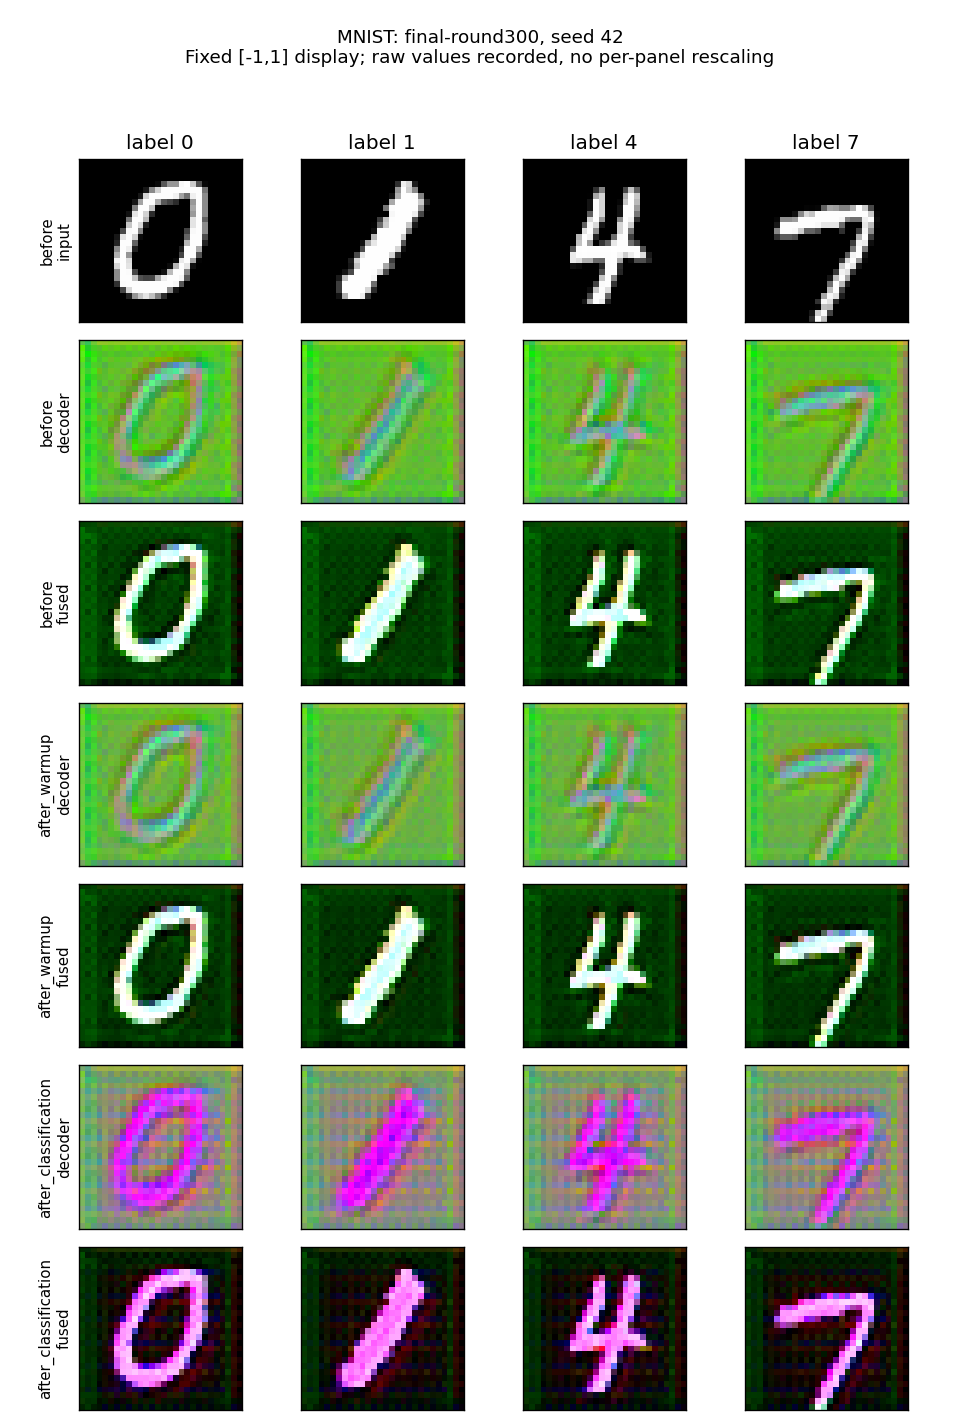
\includegraphics[width=.56in,trim=47.4bp 663.0bp 430.2bp 95.4bp,clip]{figures/digits/final-round300-MNIST.png} & 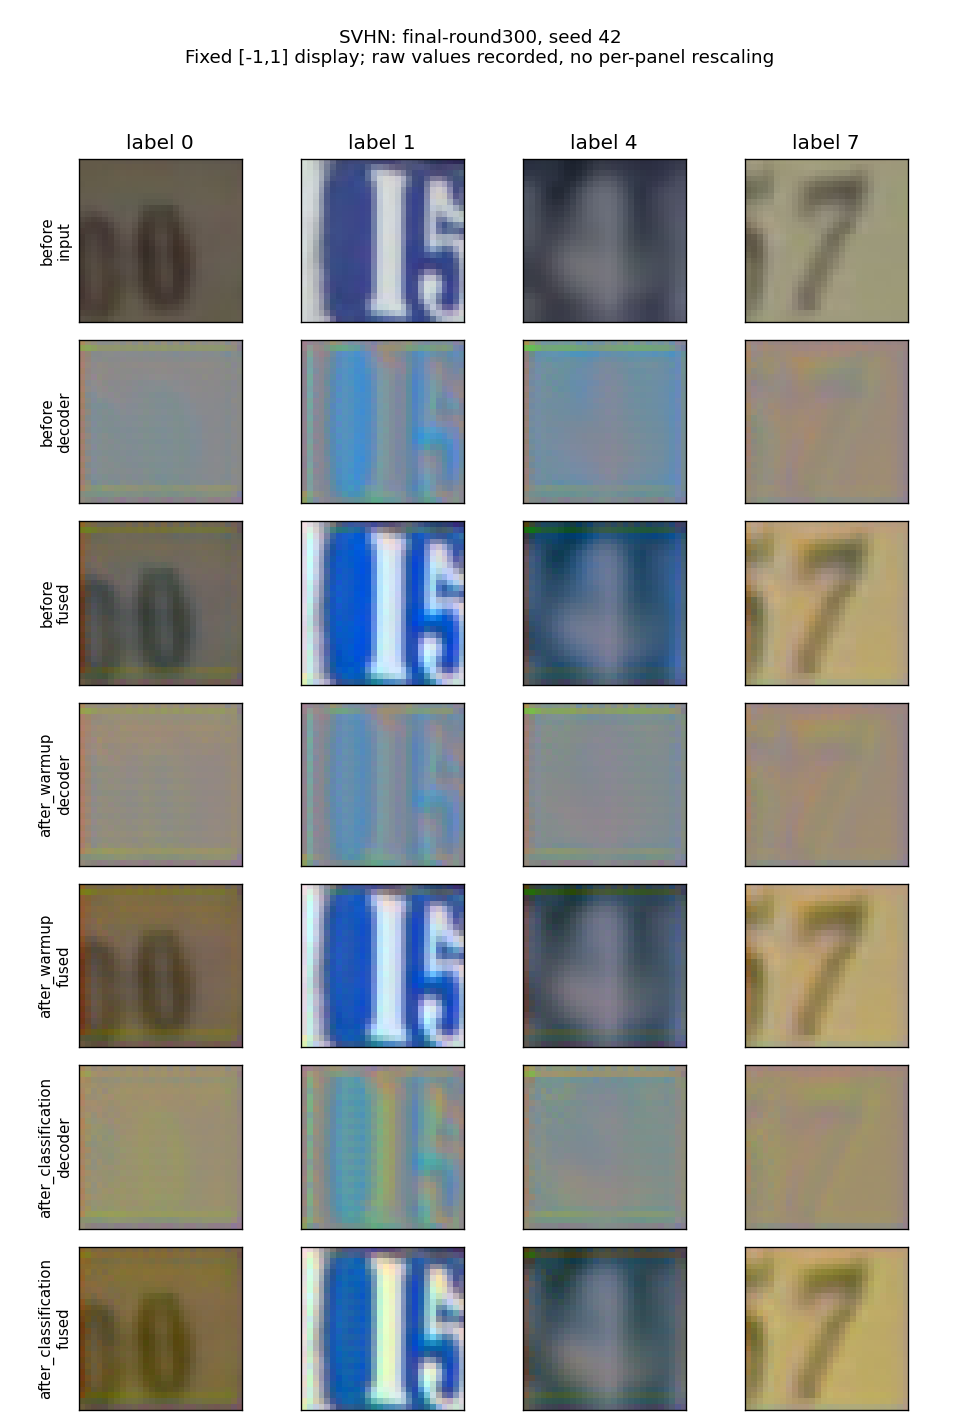
\includegraphics[width=.56in,trim=47.4bp 663.0bp 430.2bp 95.4bp,clip]{figures/digits/final-round300-SVHN.png} & 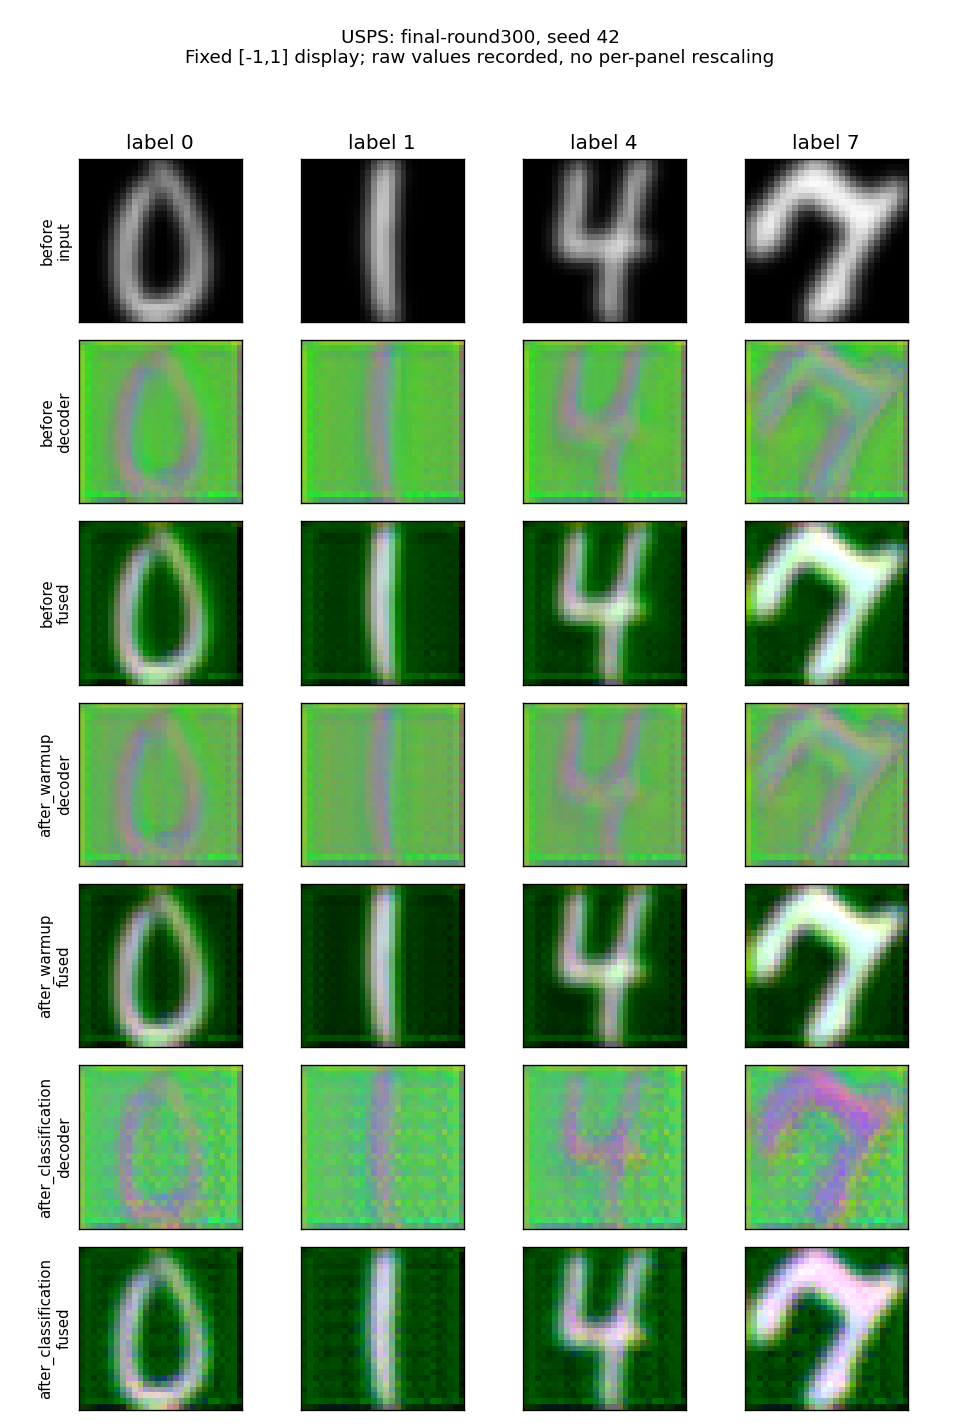
\includegraphics[width=.56in,trim=47.4bp 663.0bp 430.2bp 95.4bp,clip]{figures/digits/final-round300-USPS.png} & 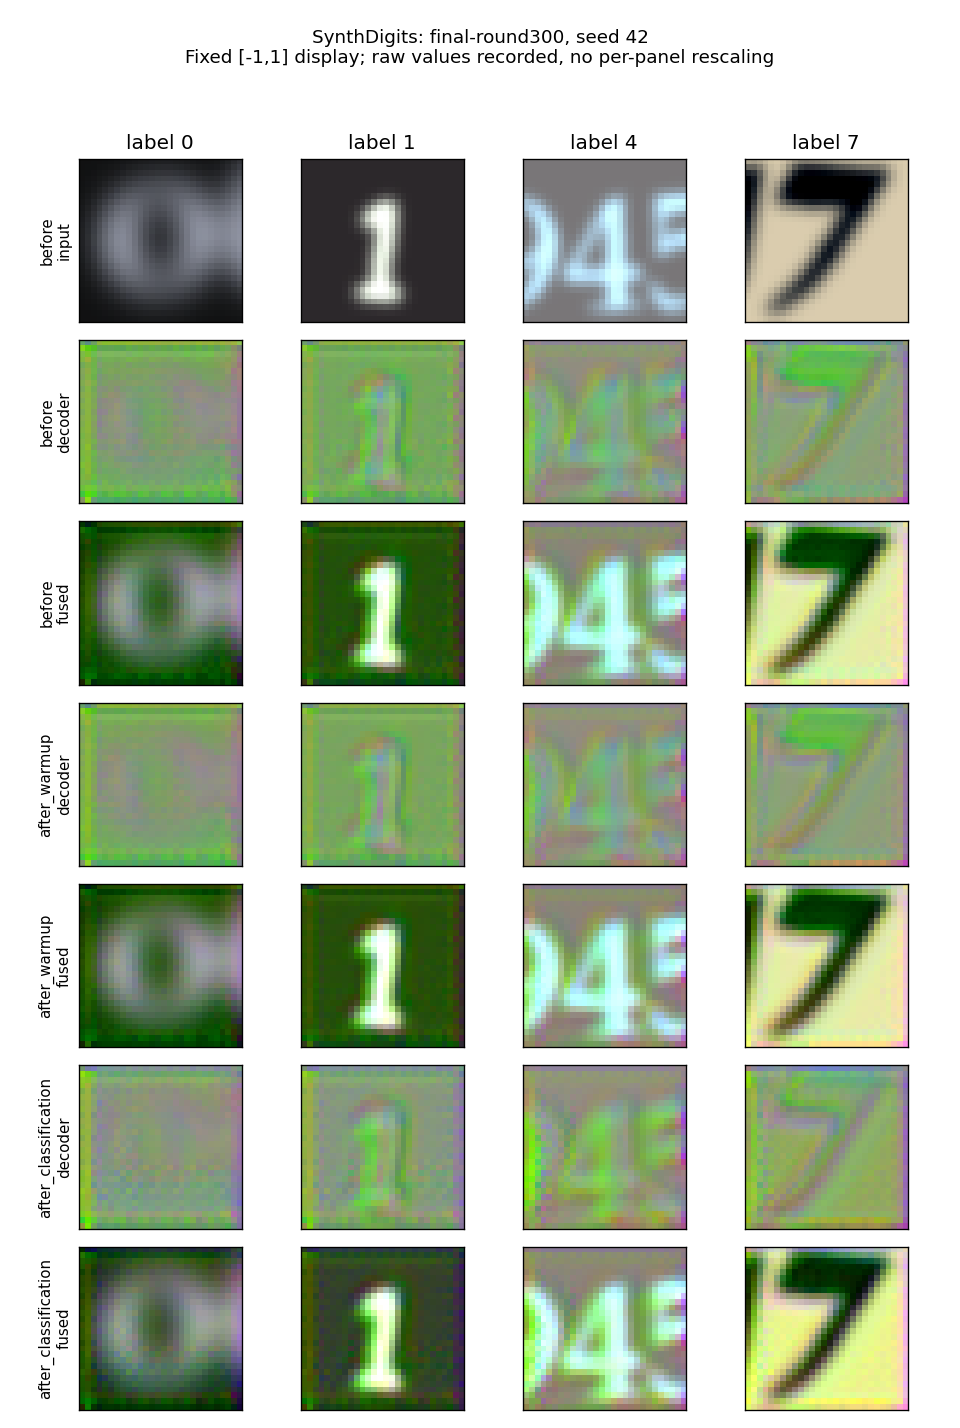
\includegraphics[width=.56in,trim=47.4bp 663.0bp 430.2bp 95.4bp,clip]{figures/digits/final-round300-SynthDigits.png} & 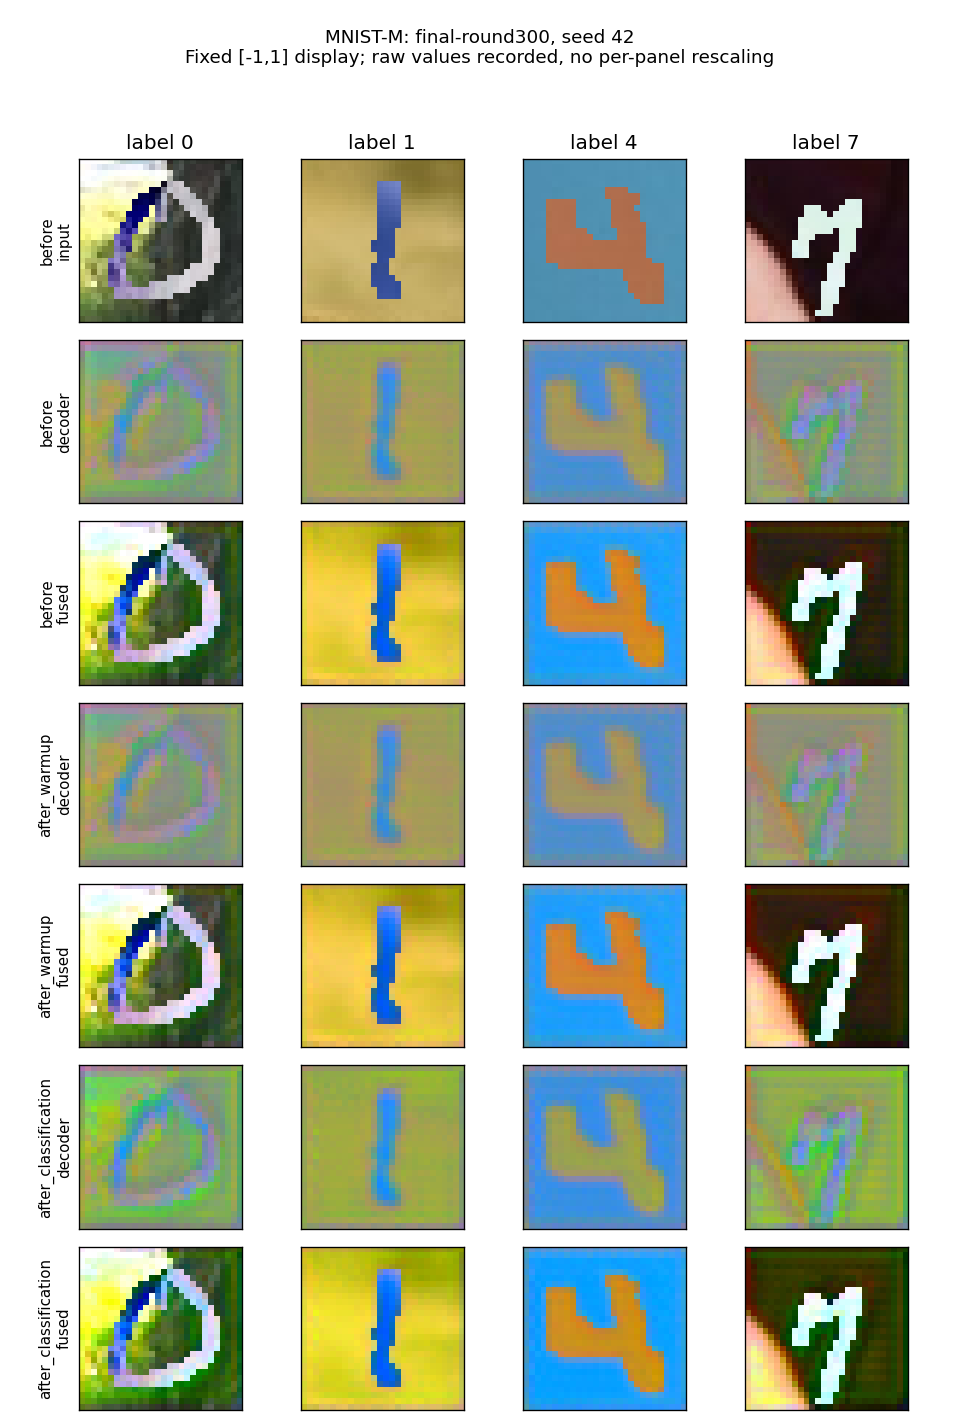
\includegraphics[width=.56in,trim=47.4bp 663.0bp 430.2bp 95.4bp,clip]{figures/digits/final-round300-MNIST-M.png} \\[-2pt]
\raisebox{.20in}{\scriptsize\shortstack[r]{Before\\decoder}} & 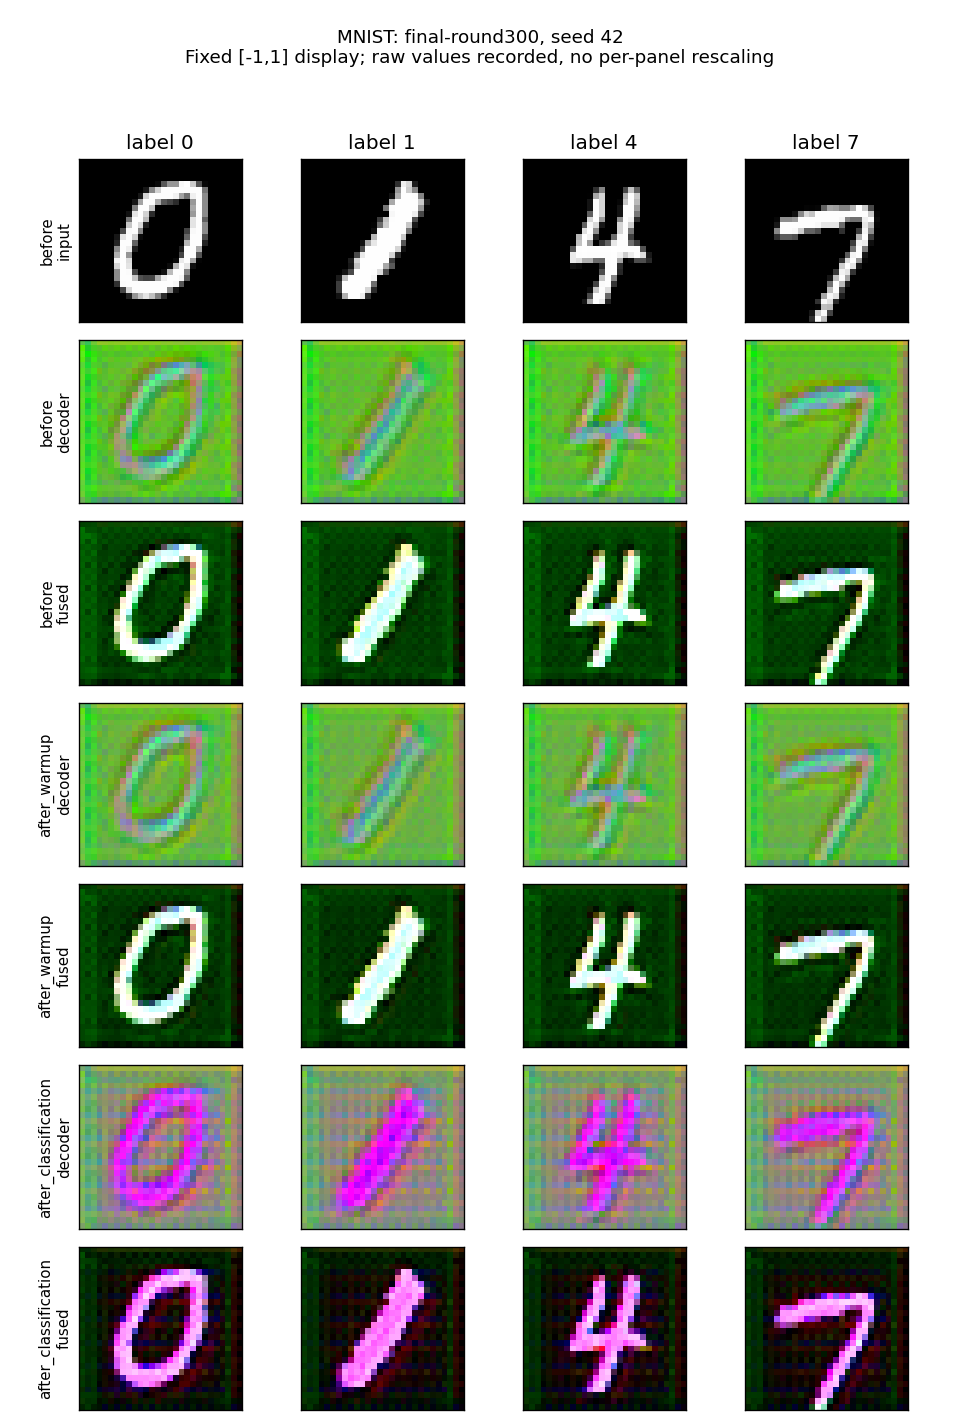
\includegraphics[width=.56in,trim=47.4bp 554.4bp 430.2bp 204.0bp,clip]{figures/digits/final-round300-MNIST.png} & 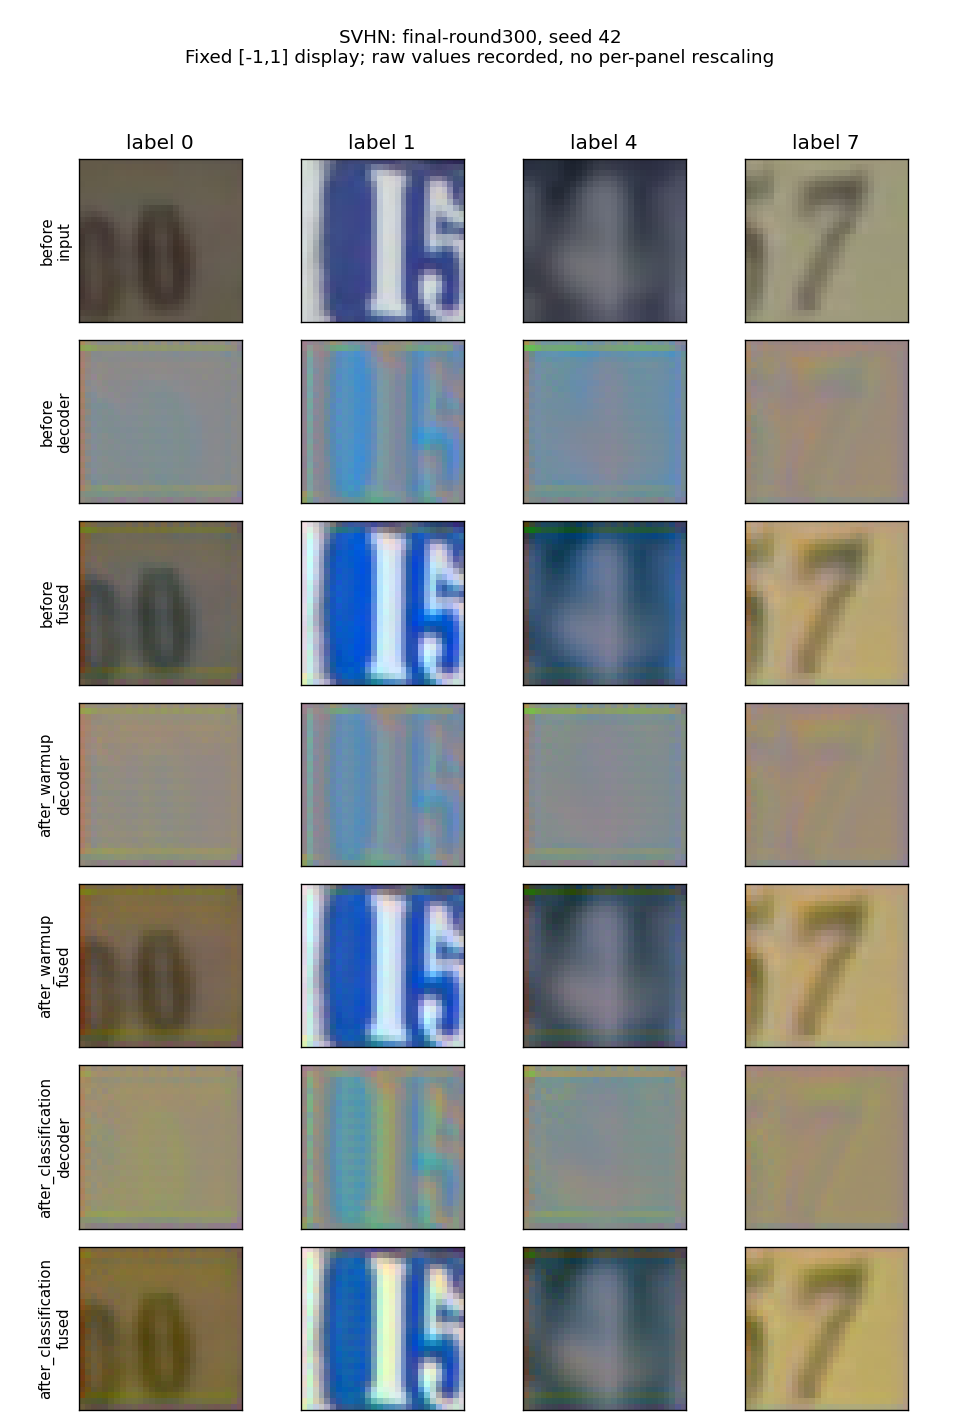
\includegraphics[width=.56in,trim=47.4bp 554.4bp 430.2bp 204.0bp,clip]{figures/digits/final-round300-SVHN.png} & 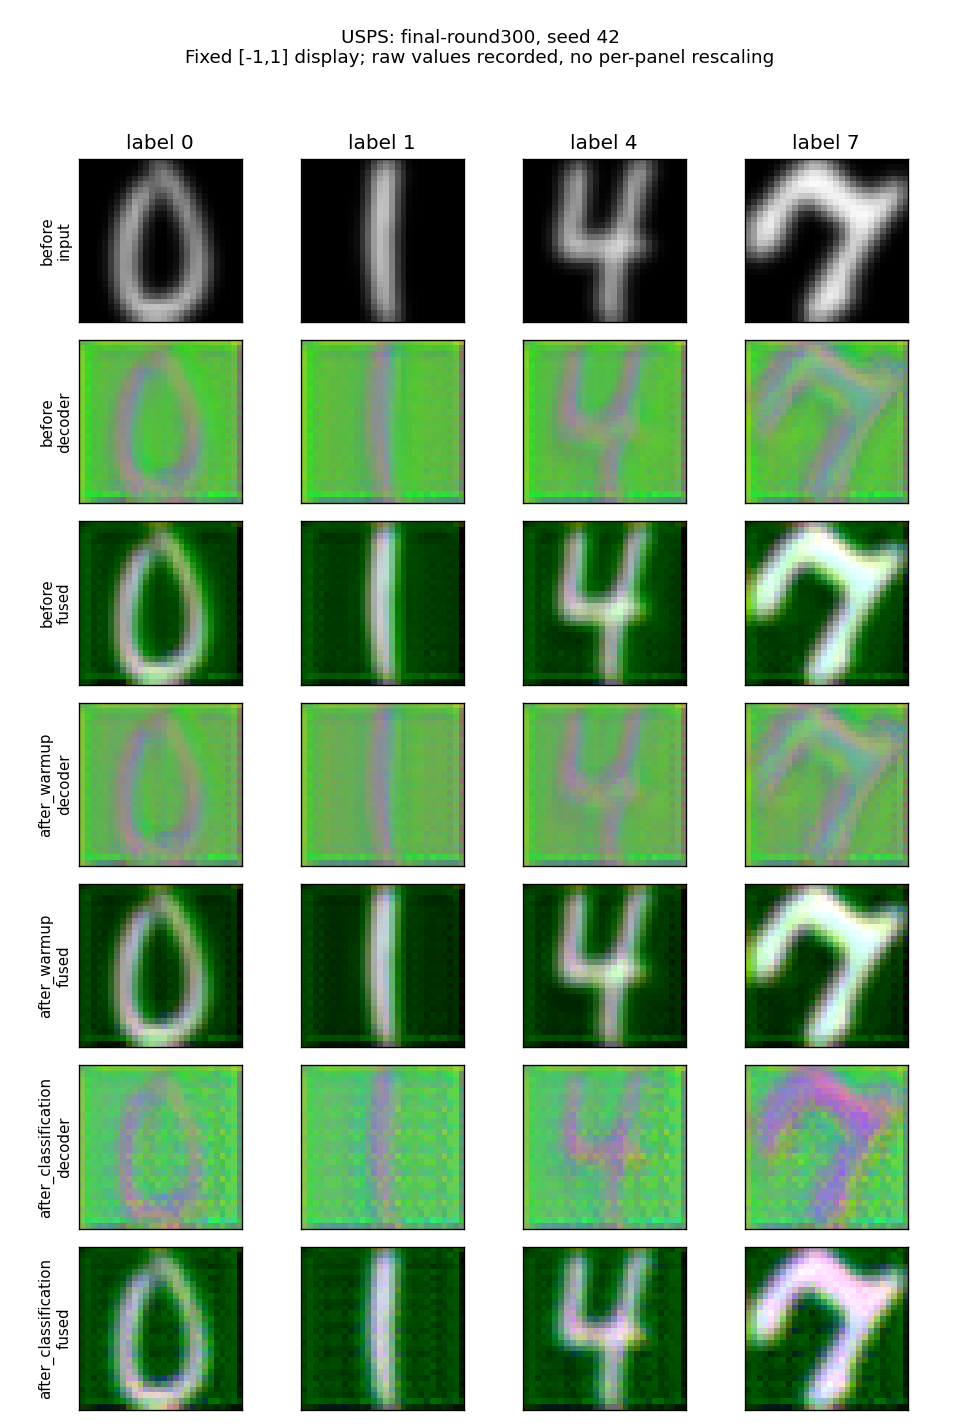
\includegraphics[width=.56in,trim=47.4bp 554.4bp 430.2bp 204.0bp,clip]{figures/digits/final-round300-USPS.png} & 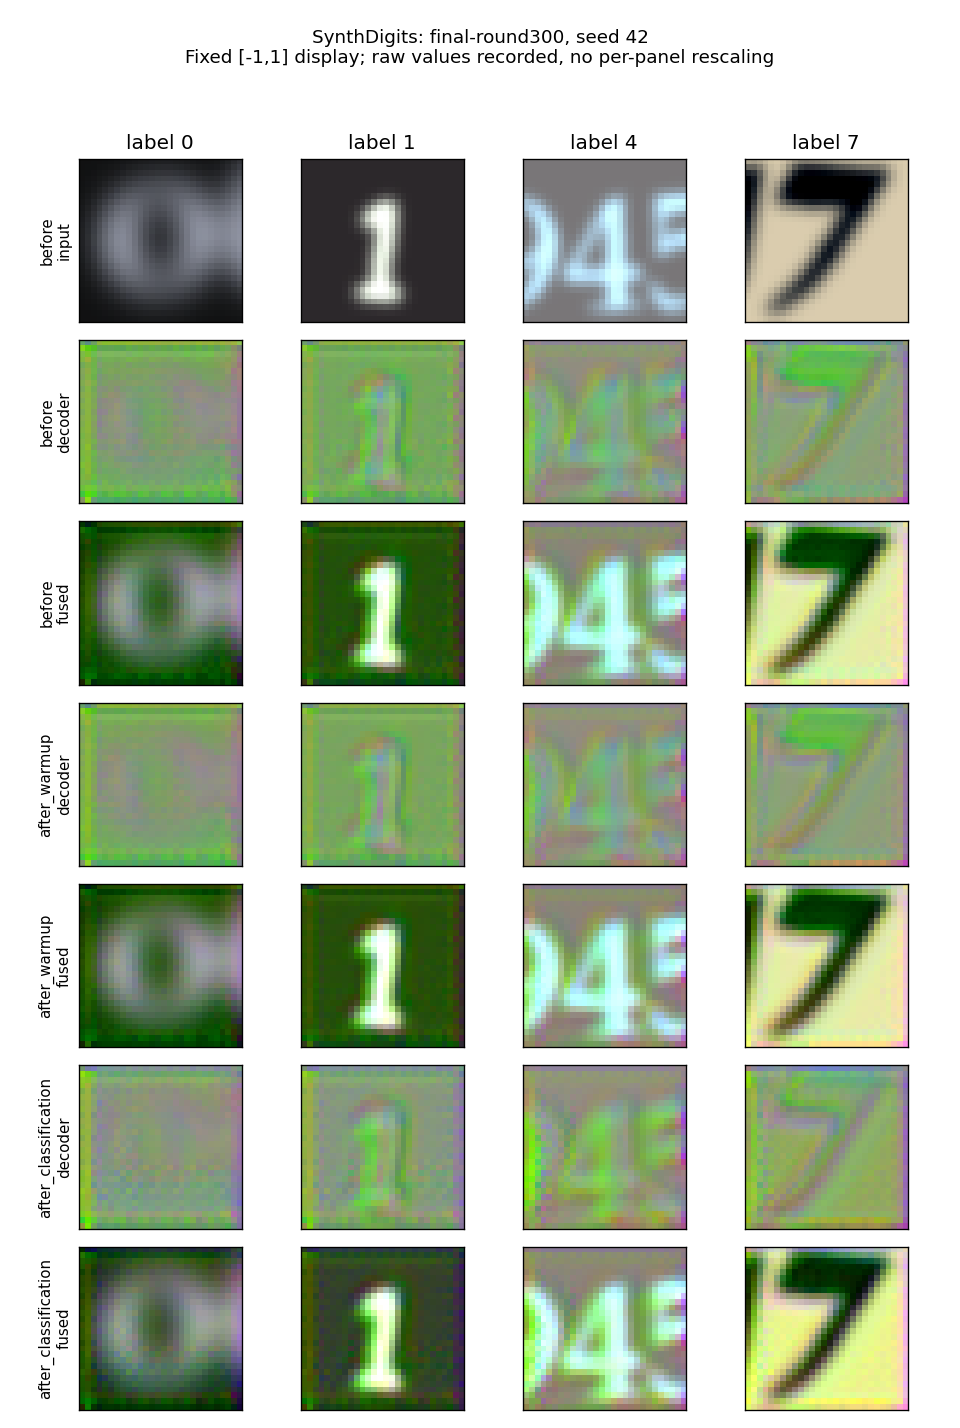
\includegraphics[width=.56in,trim=47.4bp 554.4bp 430.2bp 204.0bp,clip]{figures/digits/final-round300-SynthDigits.png} & 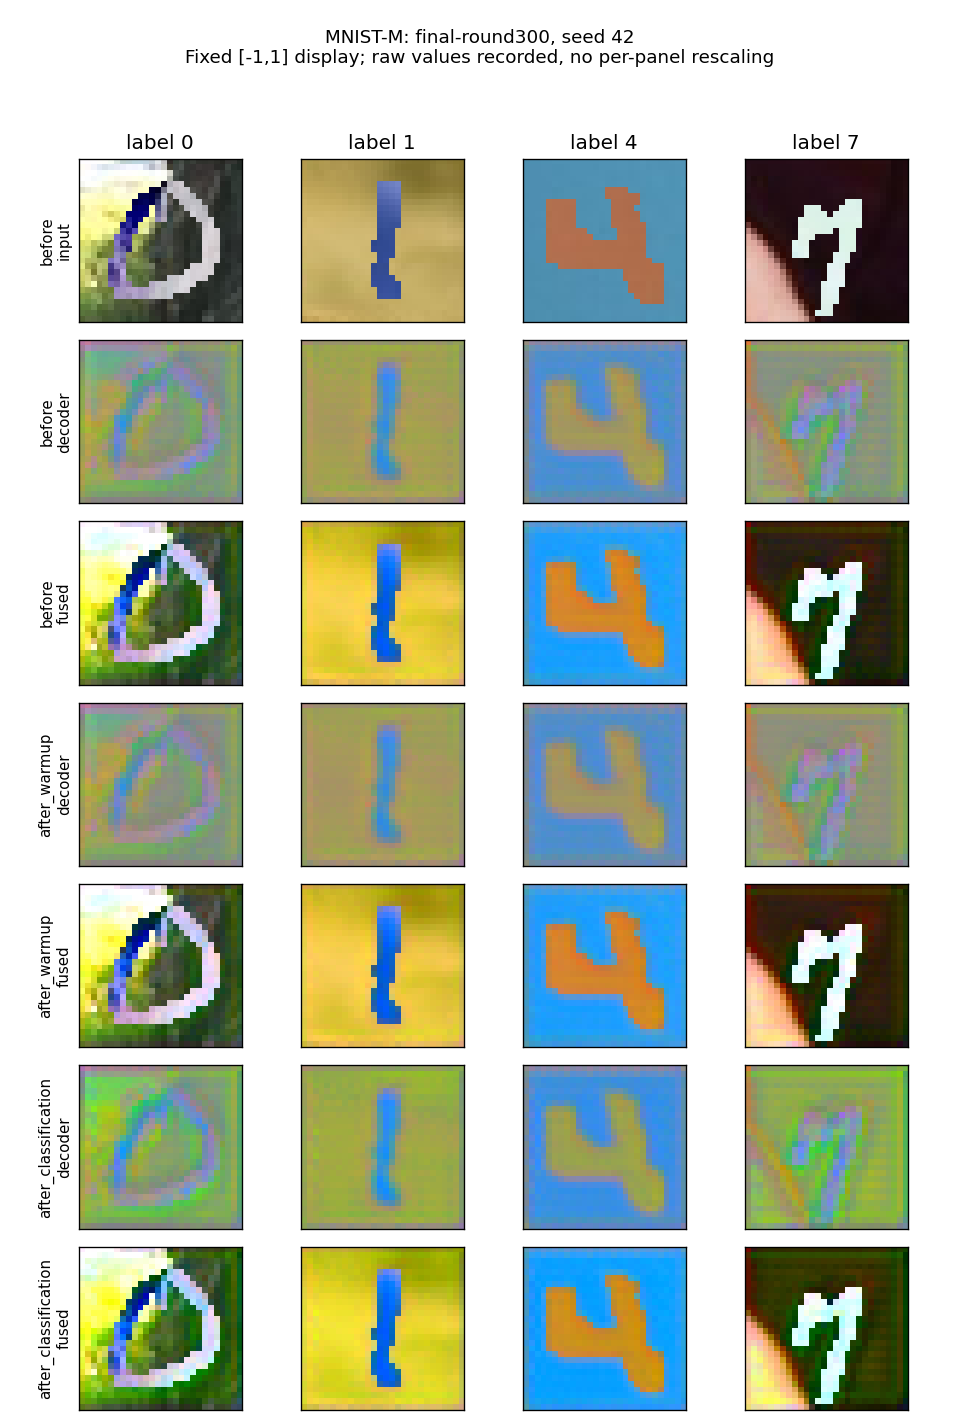
\includegraphics[width=.56in,trim=47.4bp 554.4bp 430.2bp 204.0bp,clip]{figures/digits/final-round300-MNIST-M.png} \\[-2pt]
\raisebox{.20in}{\scriptsize\shortstack[r]{Before\\fused}} & 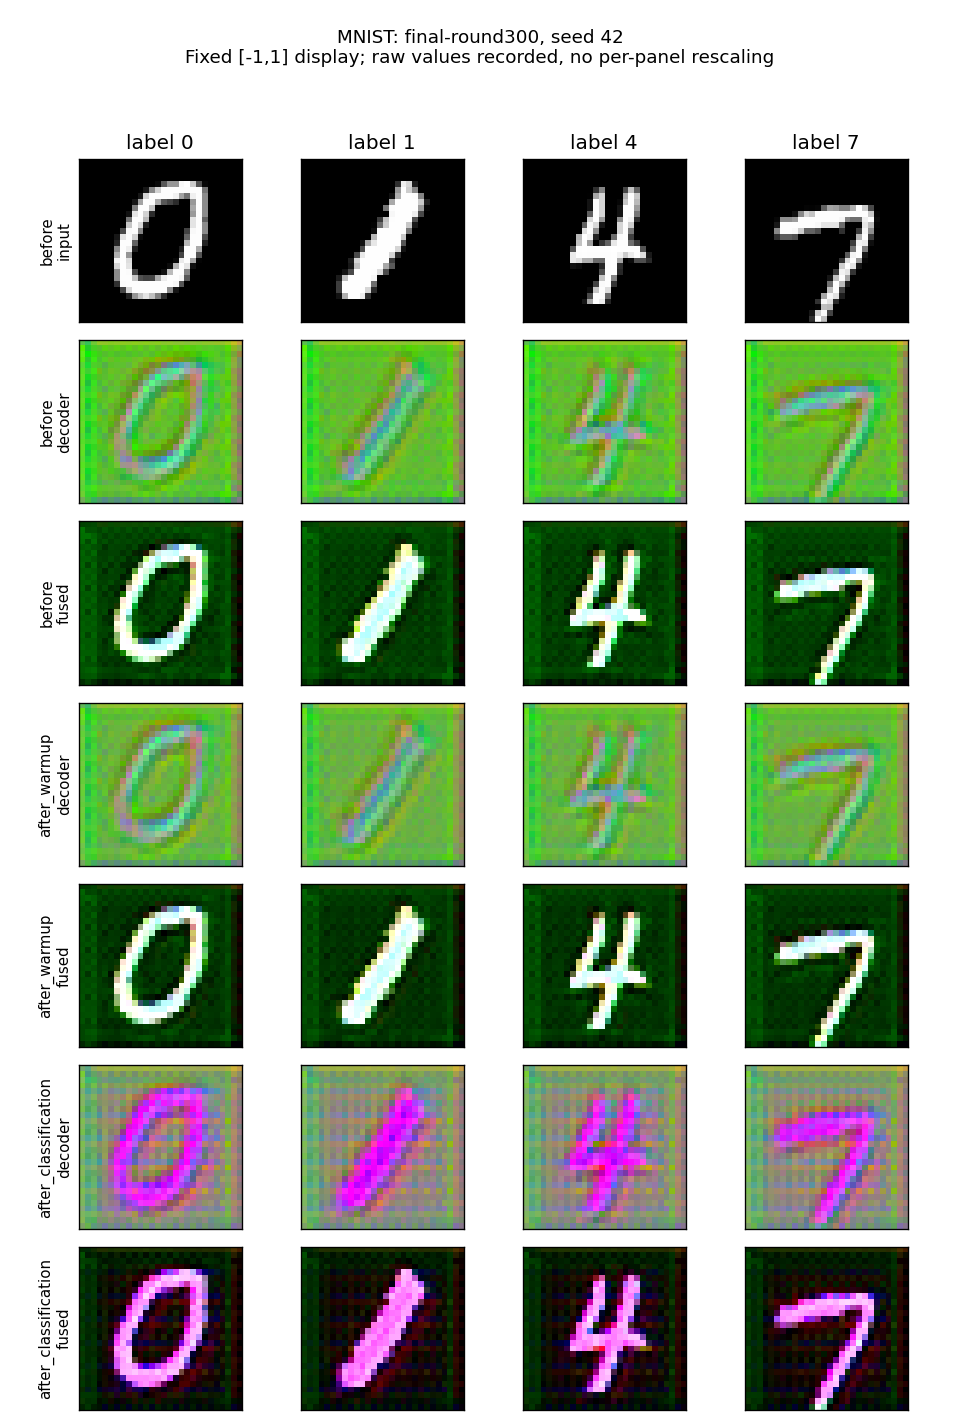
\includegraphics[width=.56in,trim=47.4bp 445.2bp 430.2bp 313.2bp,clip]{figures/digits/final-round300-MNIST.png} & 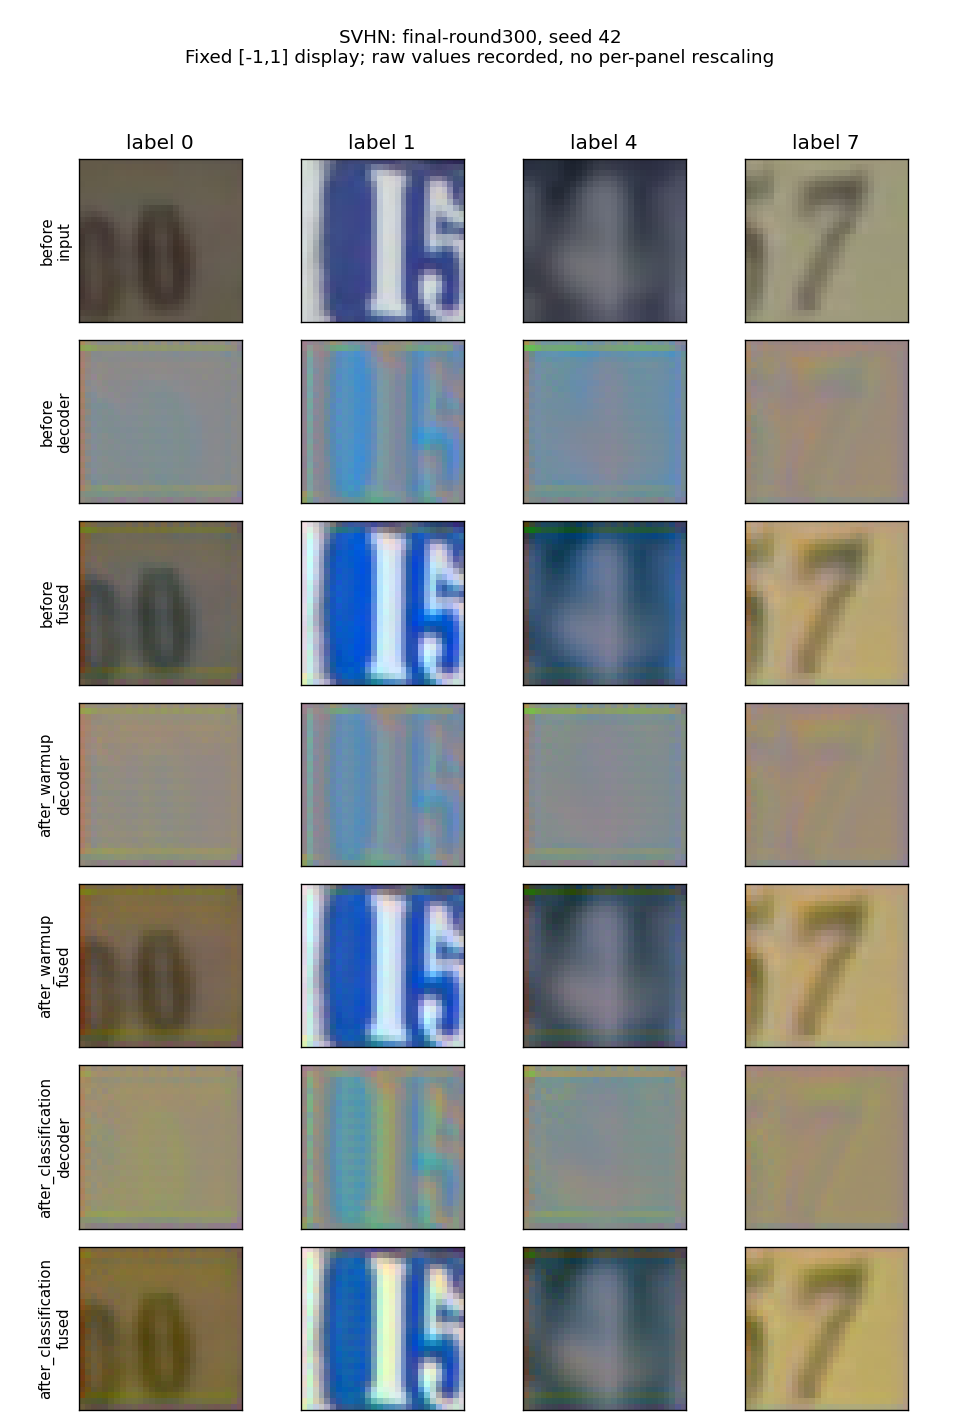
\includegraphics[width=.56in,trim=47.4bp 445.2bp 430.2bp 313.2bp,clip]{figures/digits/final-round300-SVHN.png} & 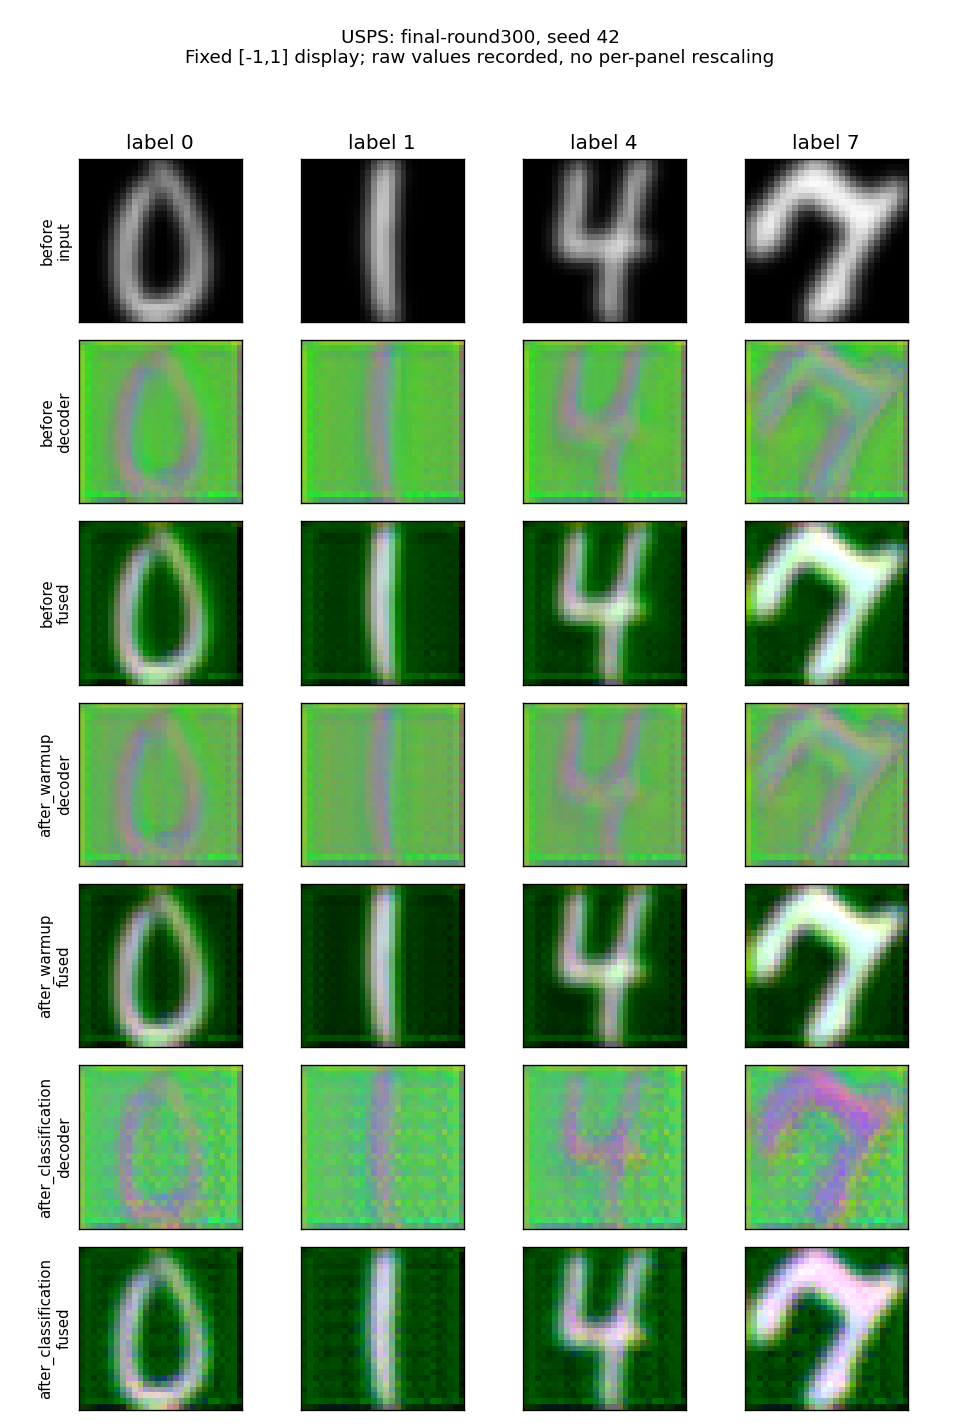
\includegraphics[width=.56in,trim=47.4bp 445.2bp 430.2bp 313.2bp,clip]{figures/digits/final-round300-USPS.png} & 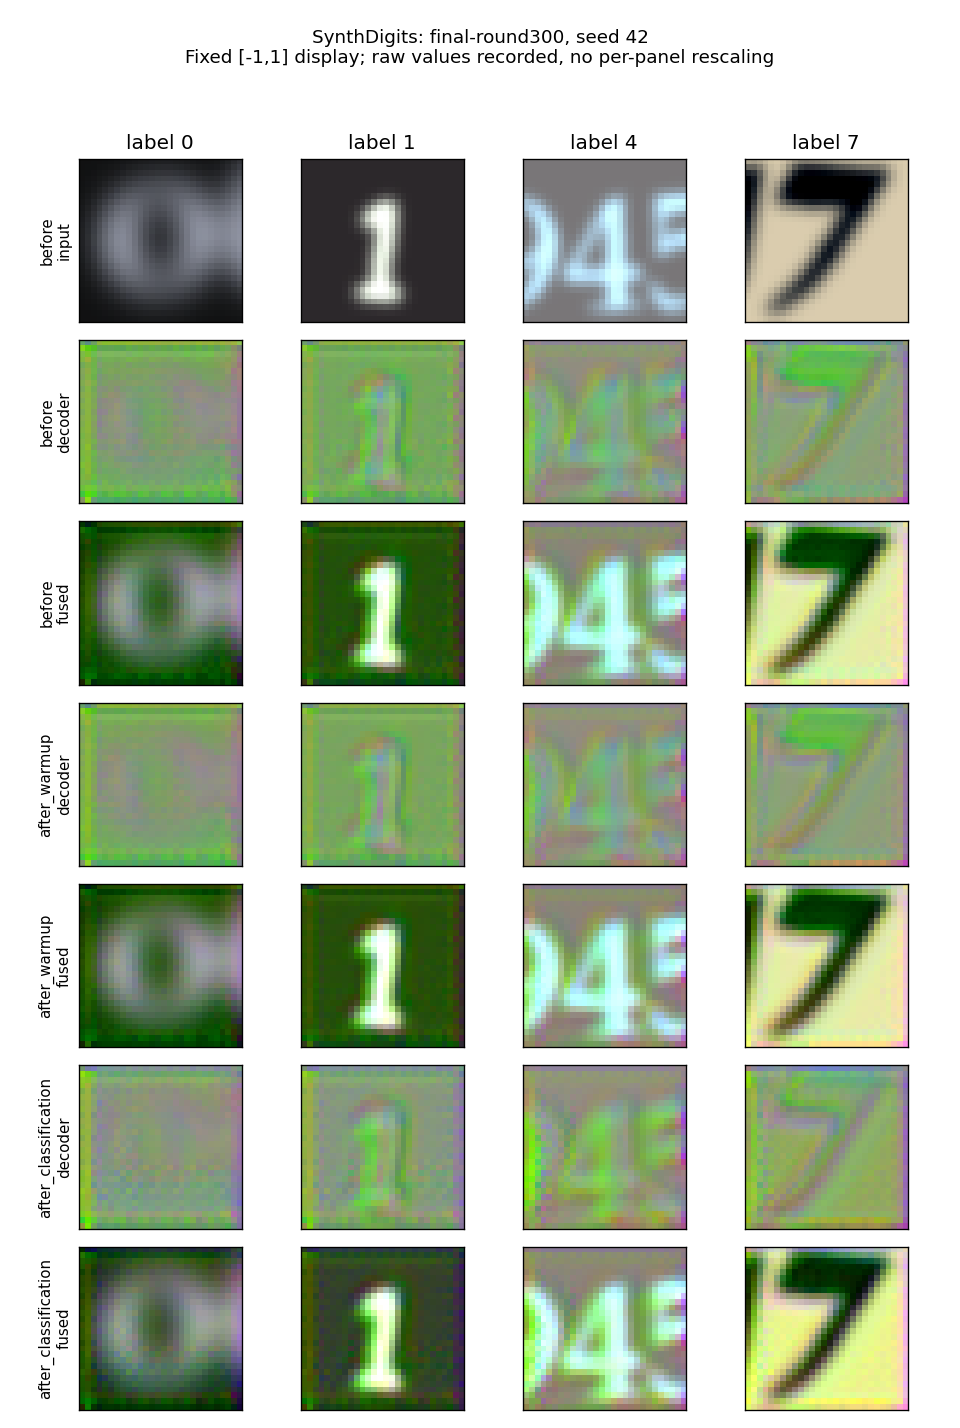
\includegraphics[width=.56in,trim=47.4bp 445.2bp 430.2bp 313.2bp,clip]{figures/digits/final-round300-SynthDigits.png} & 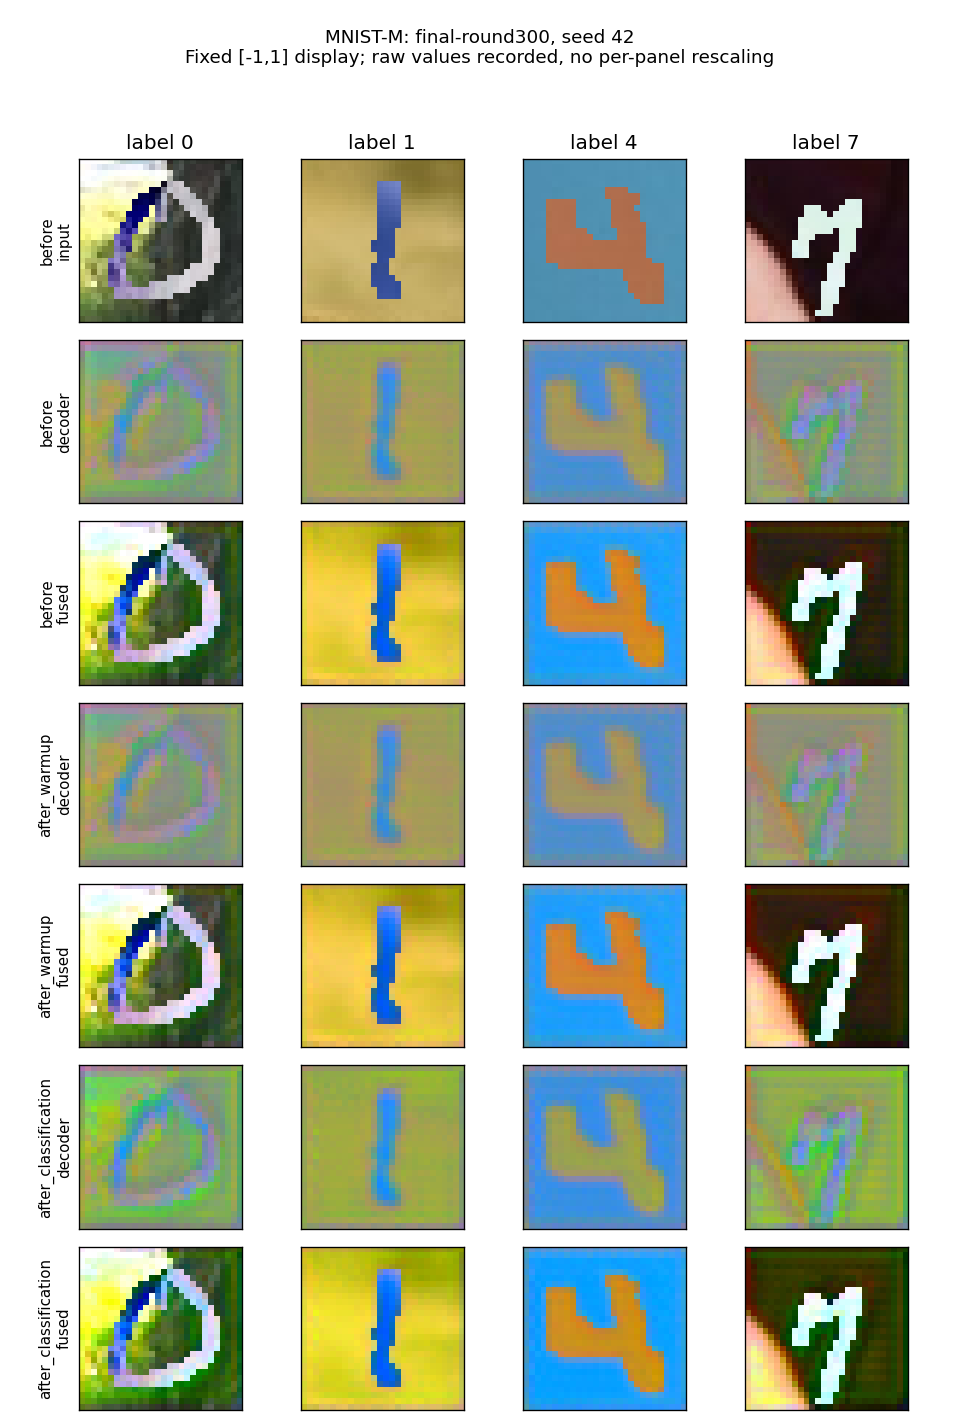
\includegraphics[width=.56in,trim=47.4bp 445.2bp 430.2bp 313.2bp,clip]{figures/digits/final-round300-MNIST-M.png} \\[-2pt]
\raisebox{.20in}{\scriptsize\shortstack[r]{After warm-up\\decoder}} & 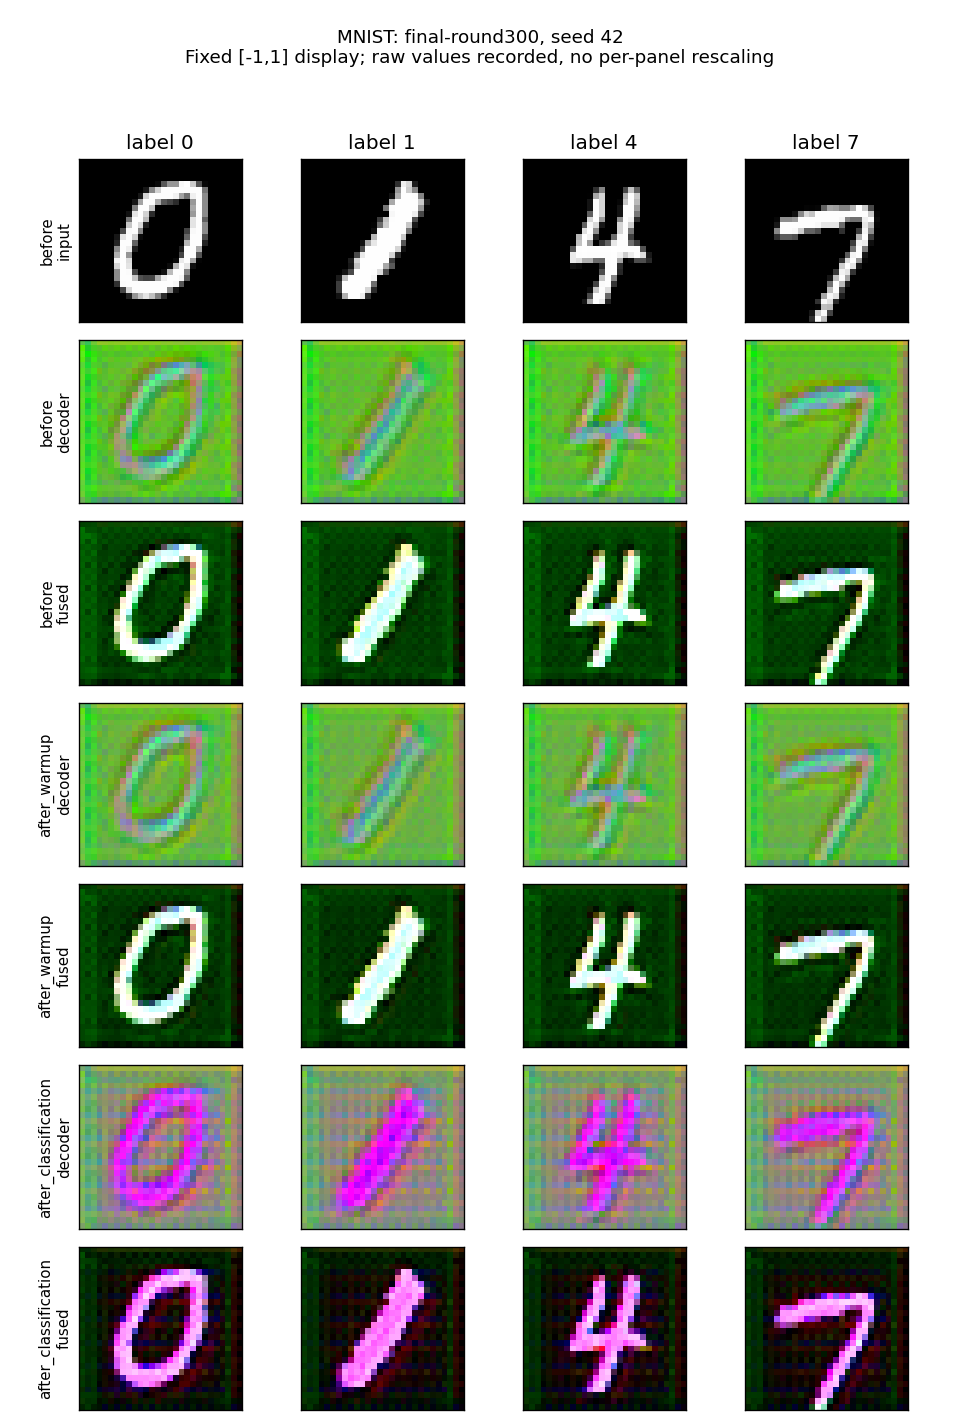
\includegraphics[width=.56in,trim=47.4bp 336.0bp 430.2bp 422.4bp,clip]{figures/digits/final-round300-MNIST.png} & 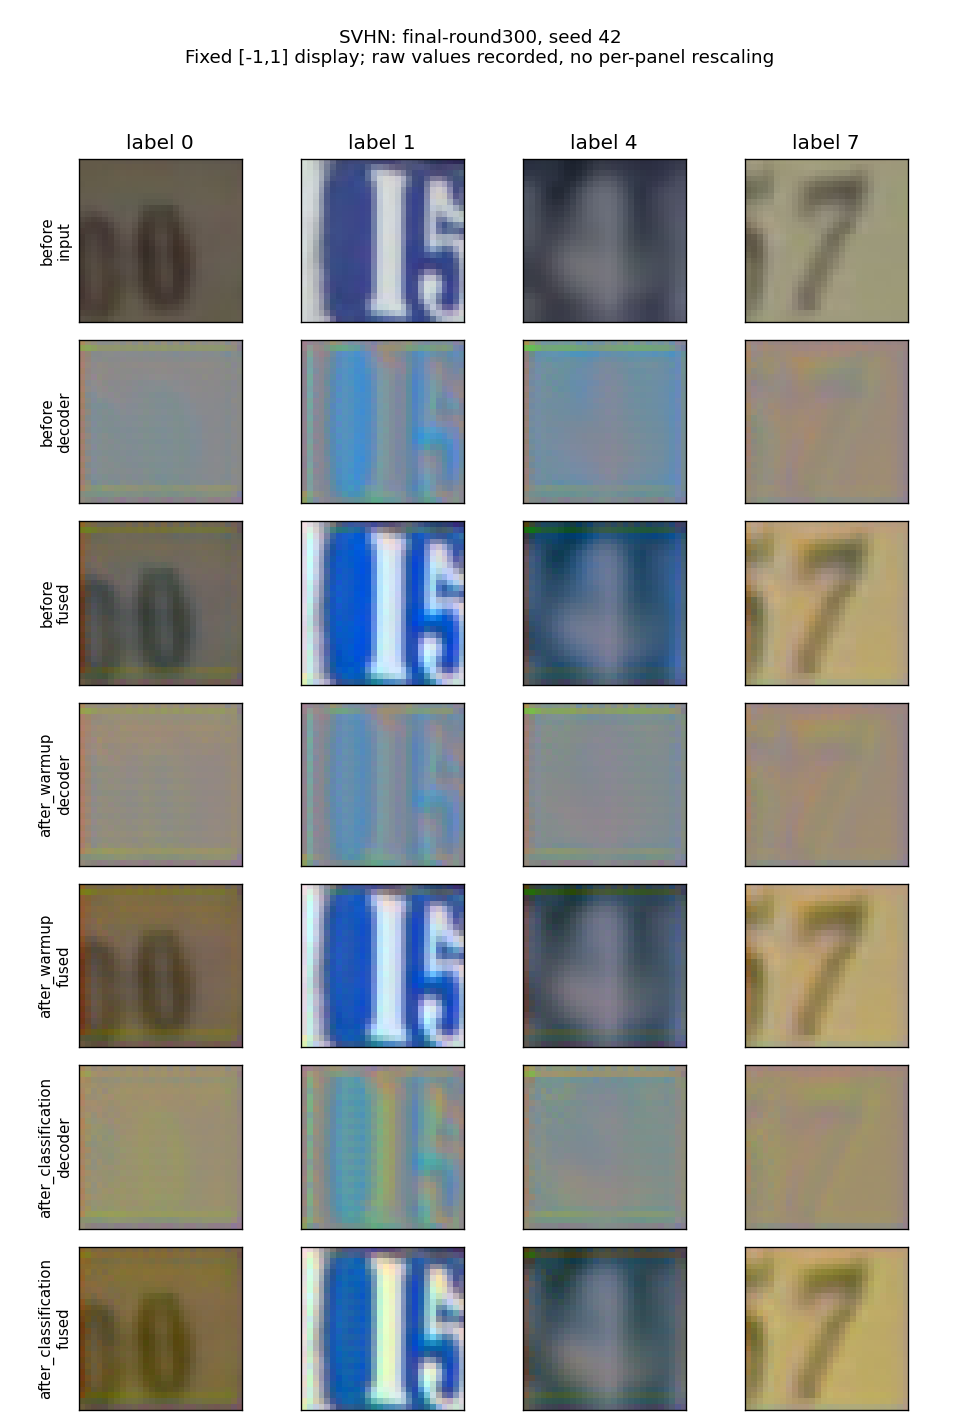
\includegraphics[width=.56in,trim=47.4bp 336.0bp 430.2bp 422.4bp,clip]{figures/digits/final-round300-SVHN.png} & 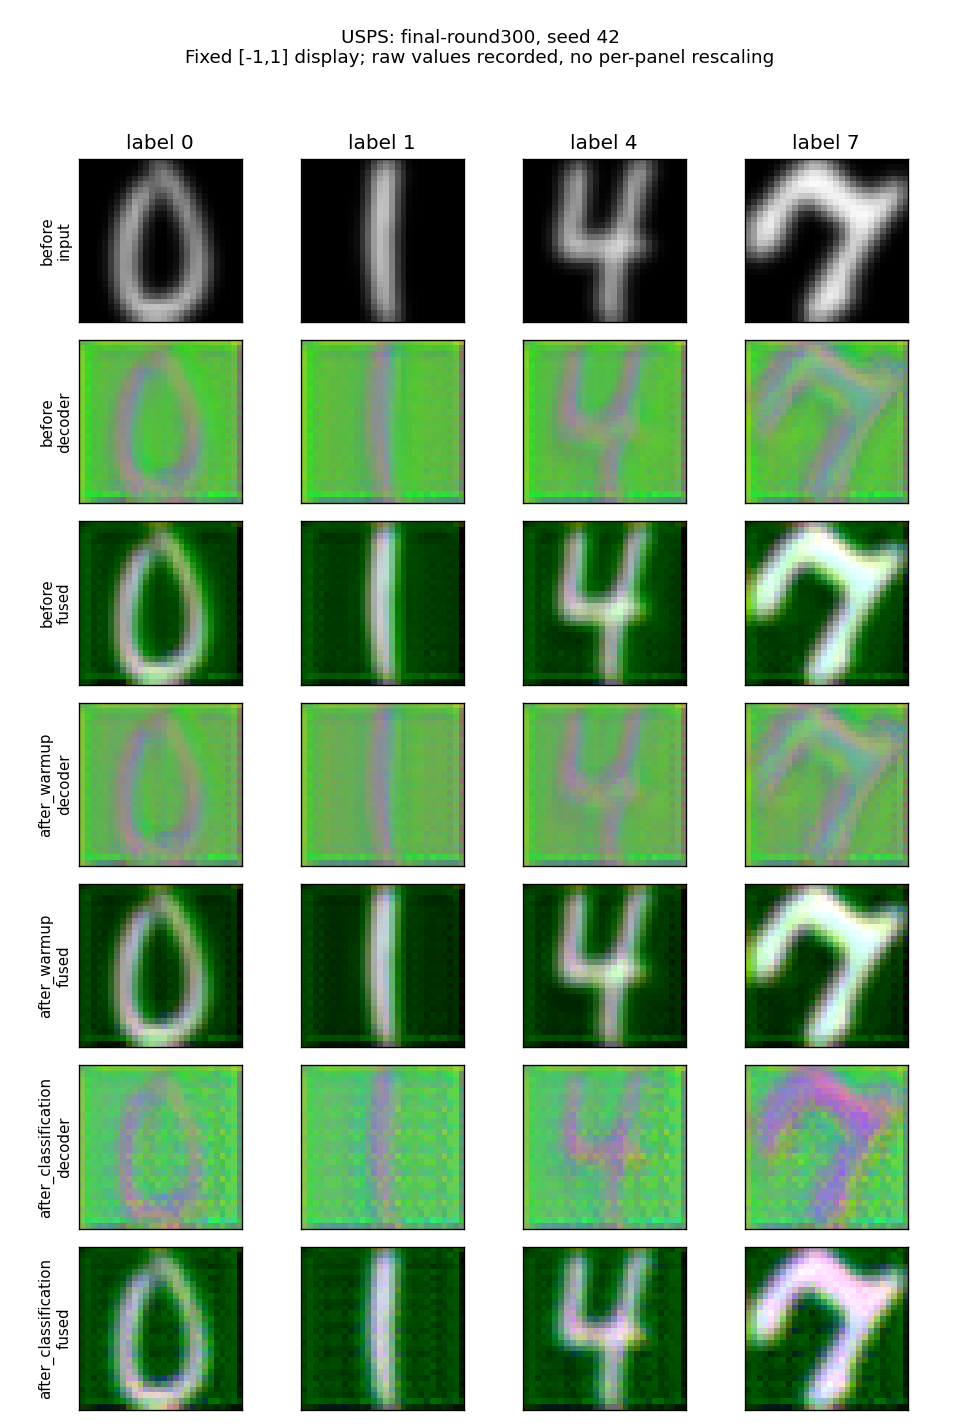
\includegraphics[width=.56in,trim=47.4bp 336.0bp 430.2bp 422.4bp,clip]{figures/digits/final-round300-USPS.png} & 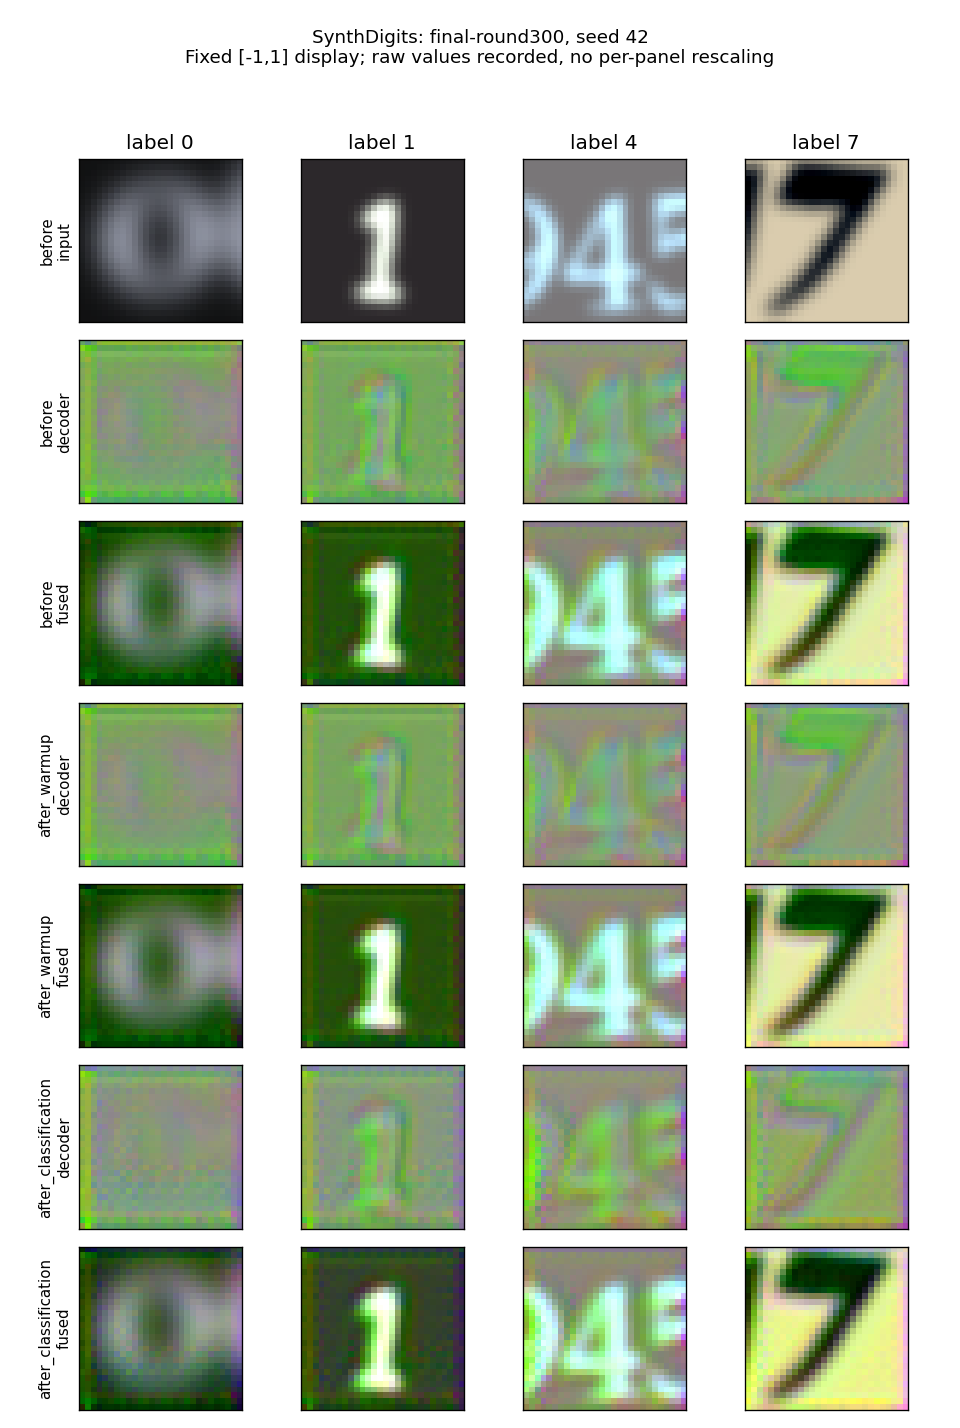
\includegraphics[width=.56in,trim=47.4bp 336.0bp 430.2bp 422.4bp,clip]{figures/digits/final-round300-SynthDigits.png} & 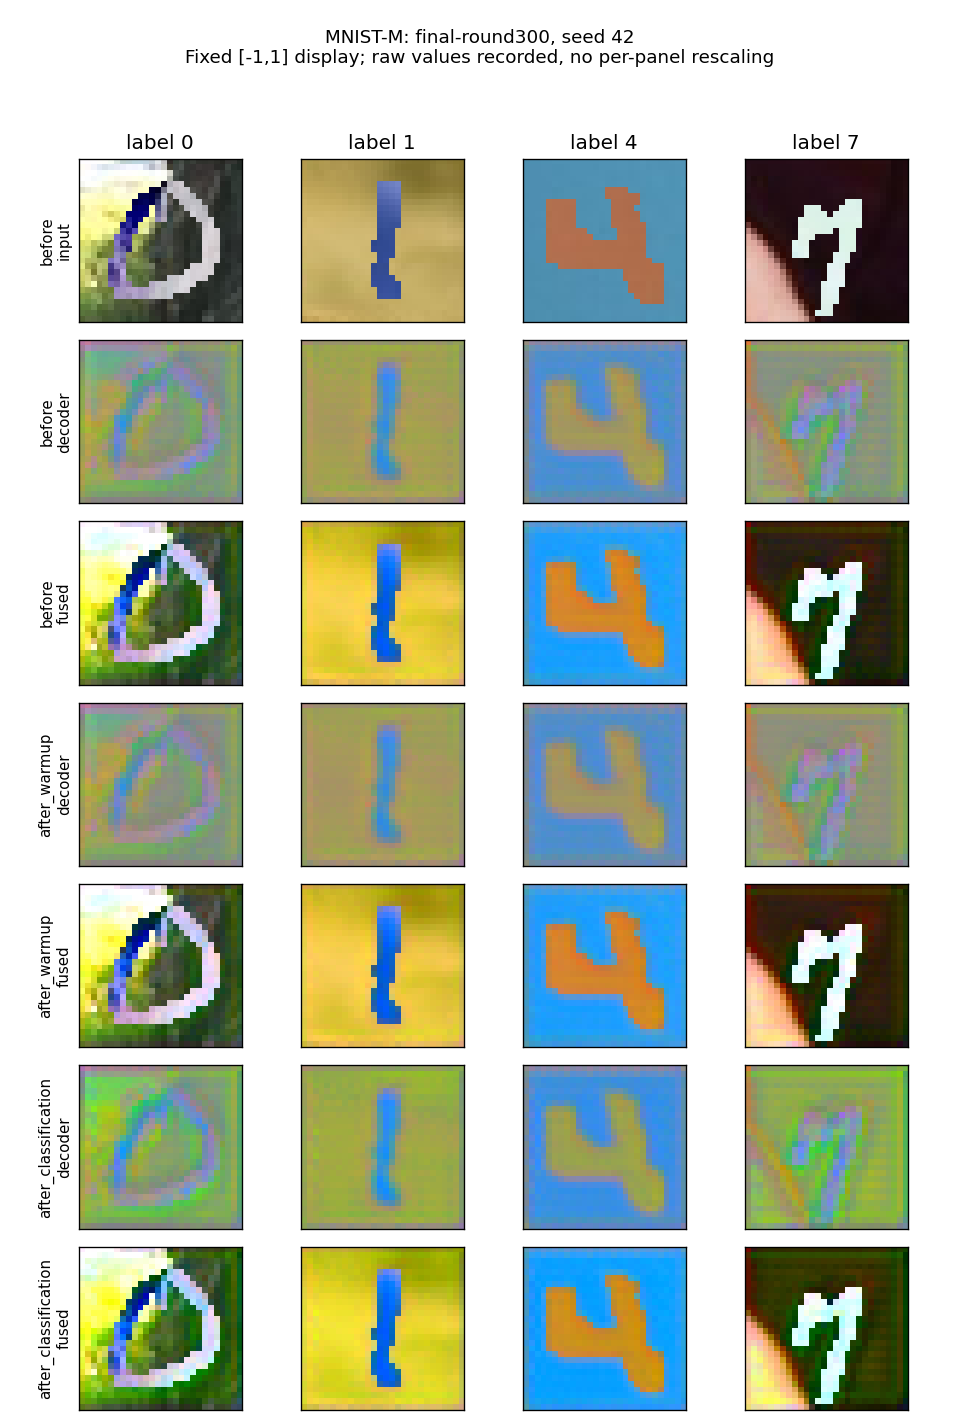
\includegraphics[width=.56in,trim=47.4bp 336.0bp 430.2bp 422.4bp,clip]{figures/digits/final-round300-MNIST-M.png} \\[-2pt]
\raisebox{.20in}{\scriptsize\shortstack[r]{After warm-up\\fused}} & 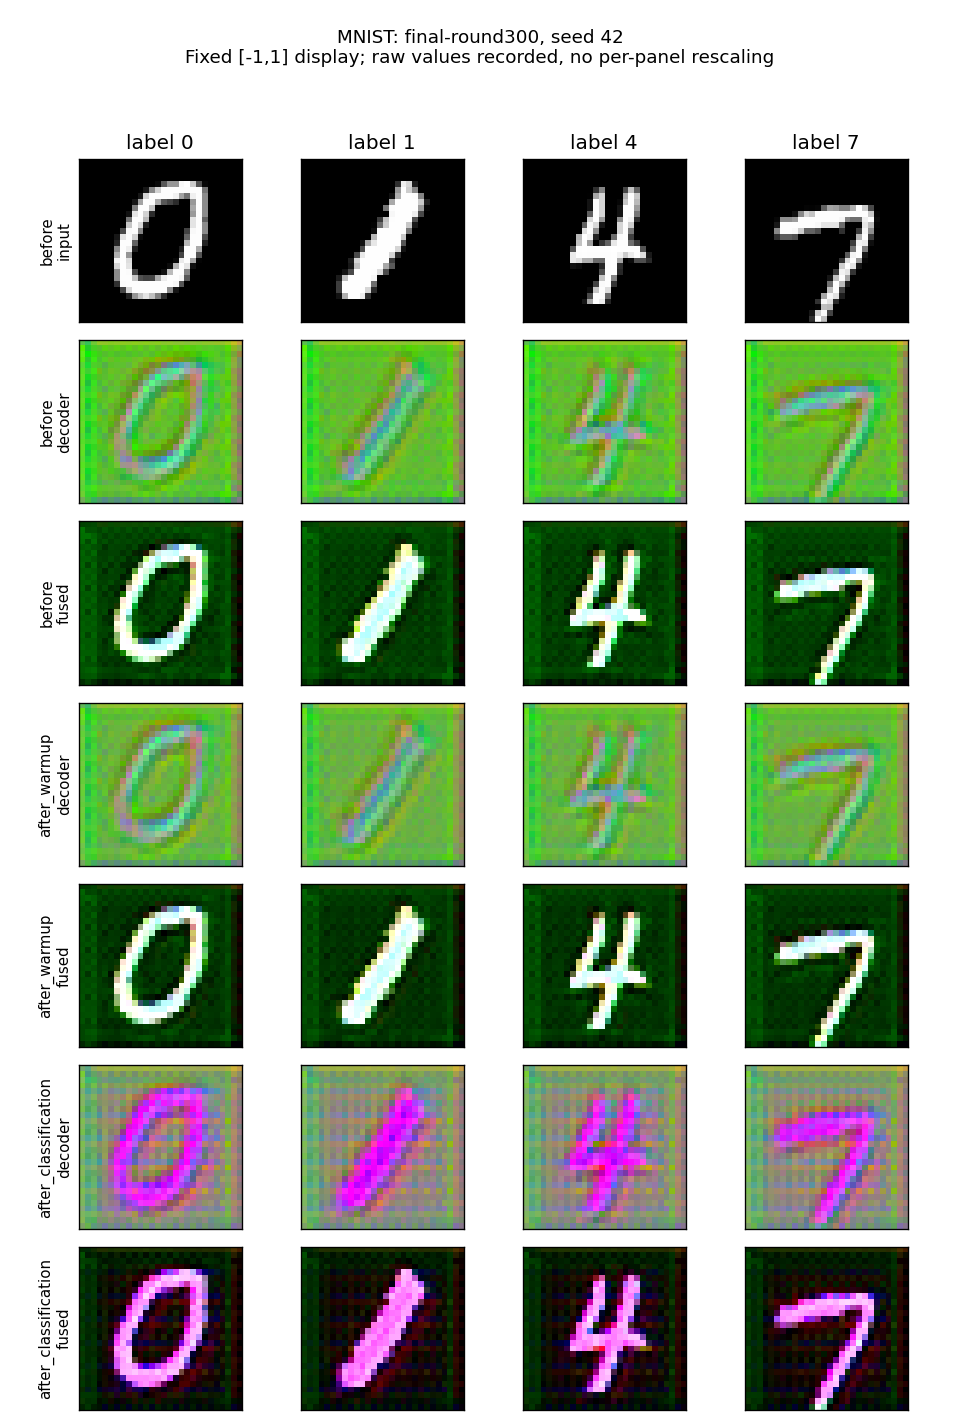
\includegraphics[width=.56in,trim=47.4bp 227.4bp 430.2bp 531.0bp,clip]{figures/digits/final-round300-MNIST.png} & 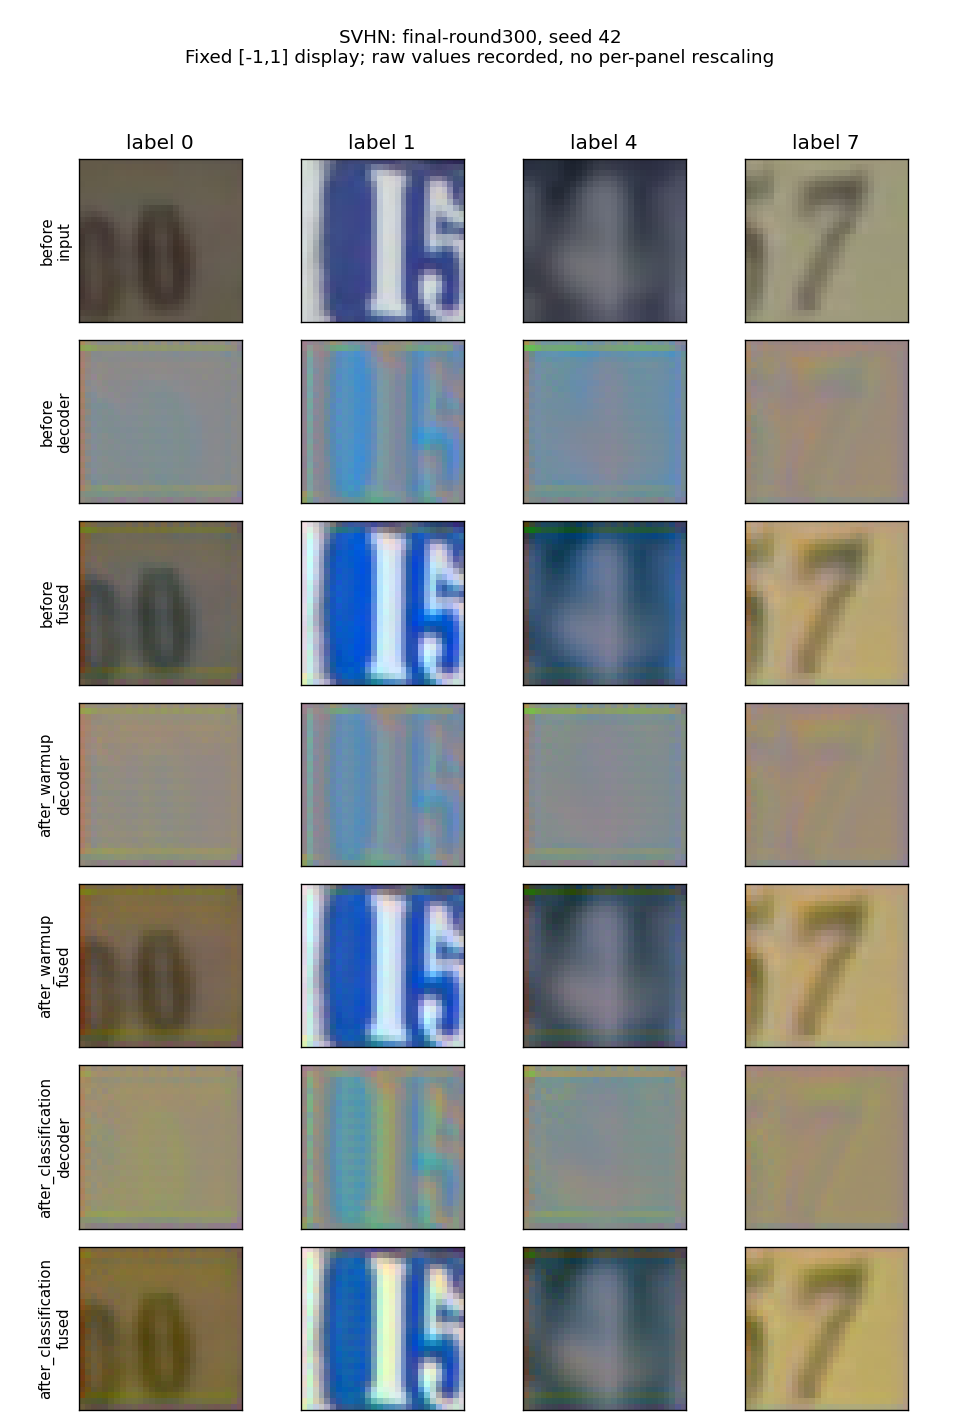
\includegraphics[width=.56in,trim=47.4bp 227.4bp 430.2bp 531.0bp,clip]{figures/digits/final-round300-SVHN.png} & 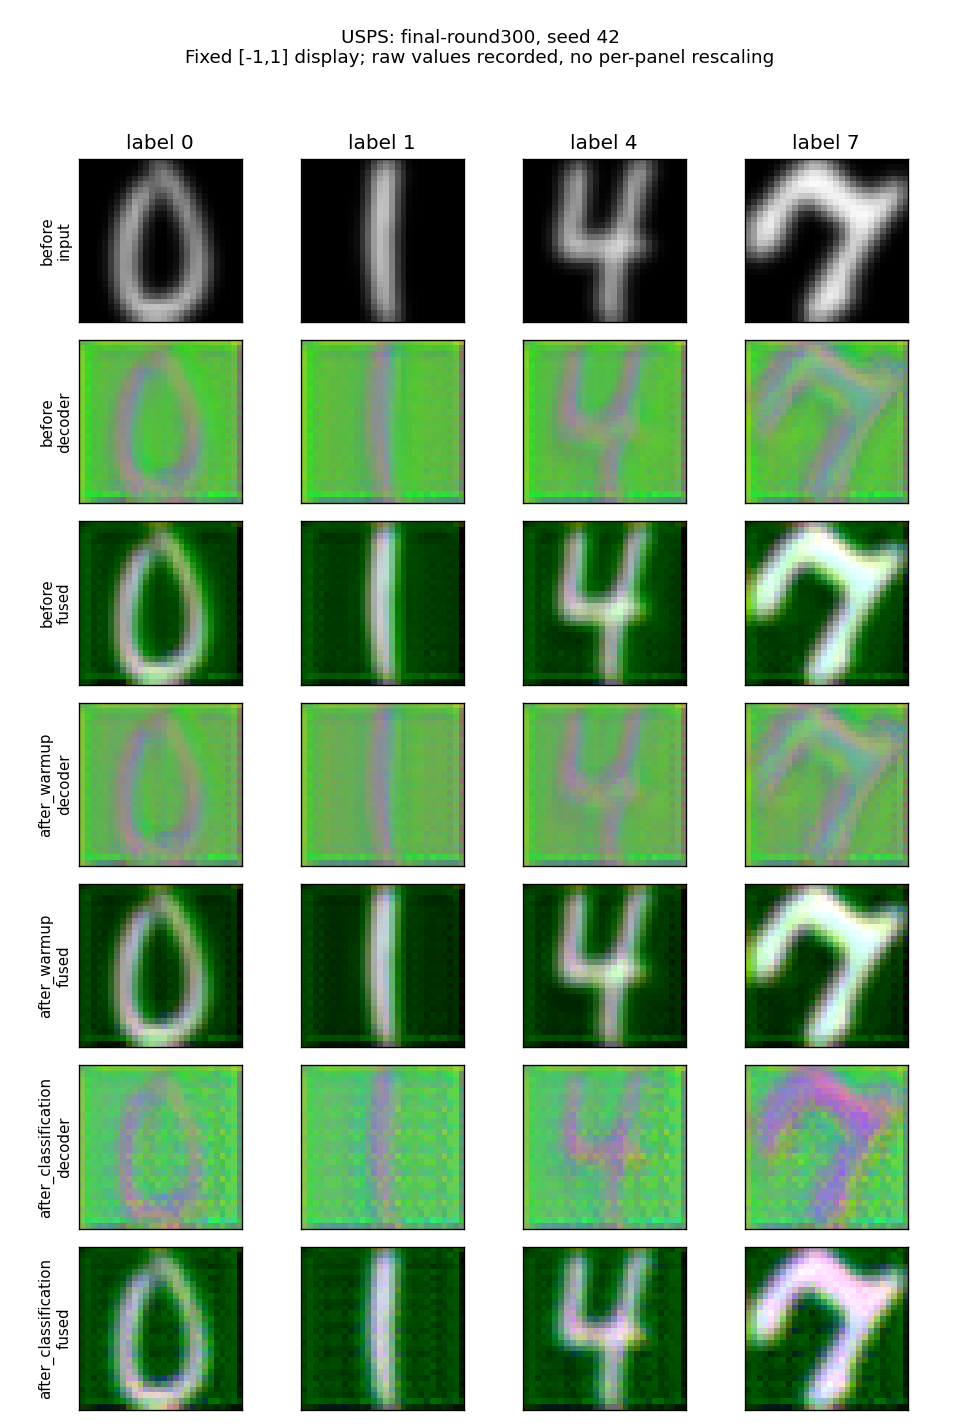
\includegraphics[width=.56in,trim=47.4bp 227.4bp 430.2bp 531.0bp,clip]{figures/digits/final-round300-USPS.png} & 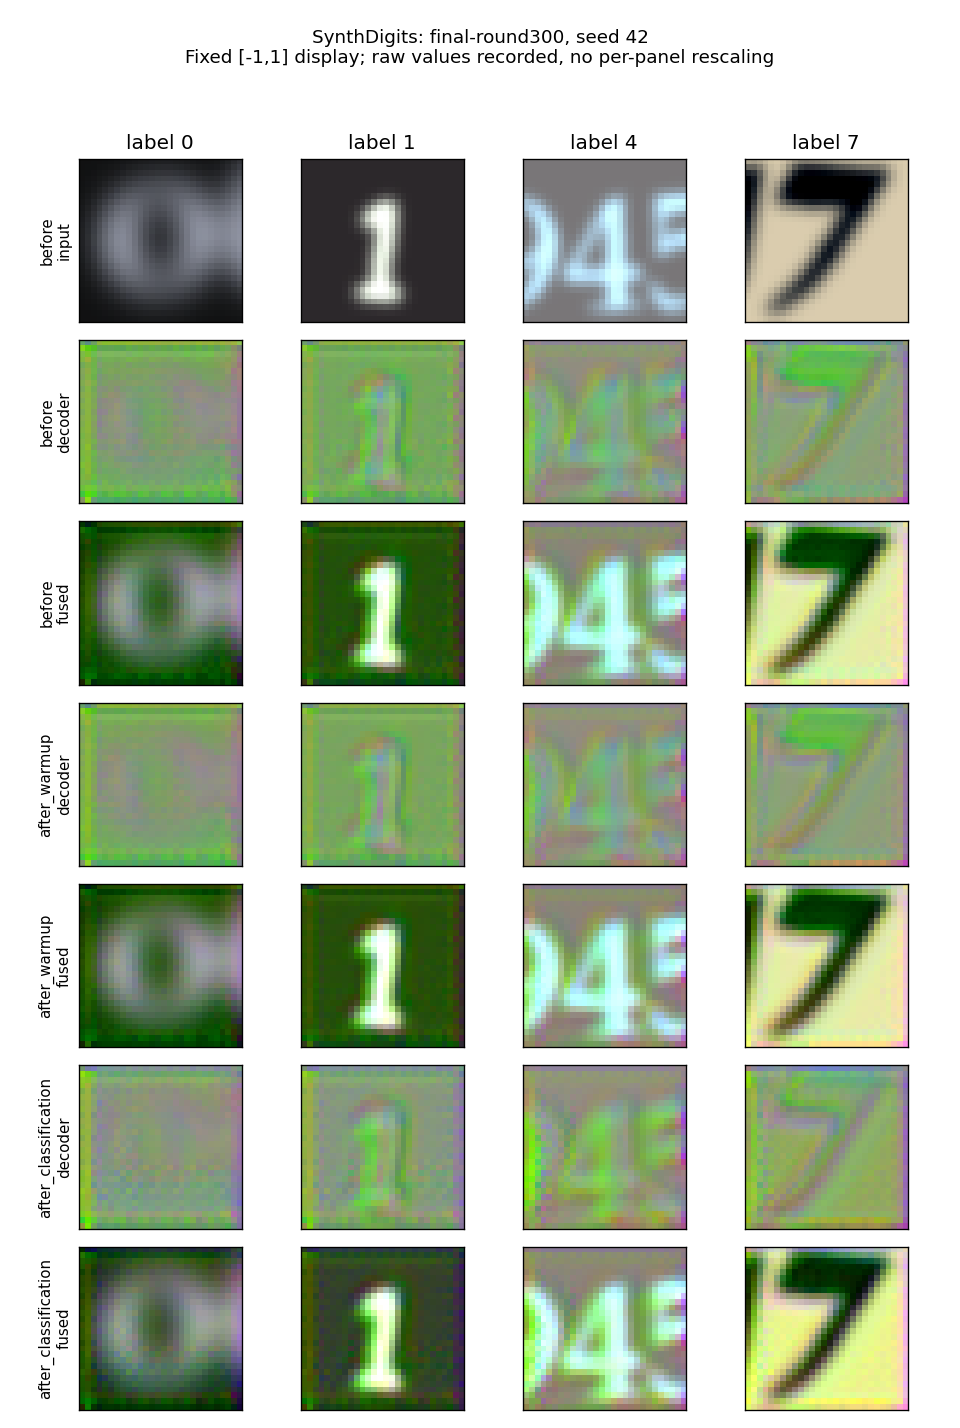
\includegraphics[width=.56in,trim=47.4bp 227.4bp 430.2bp 531.0bp,clip]{figures/digits/final-round300-SynthDigits.png} & 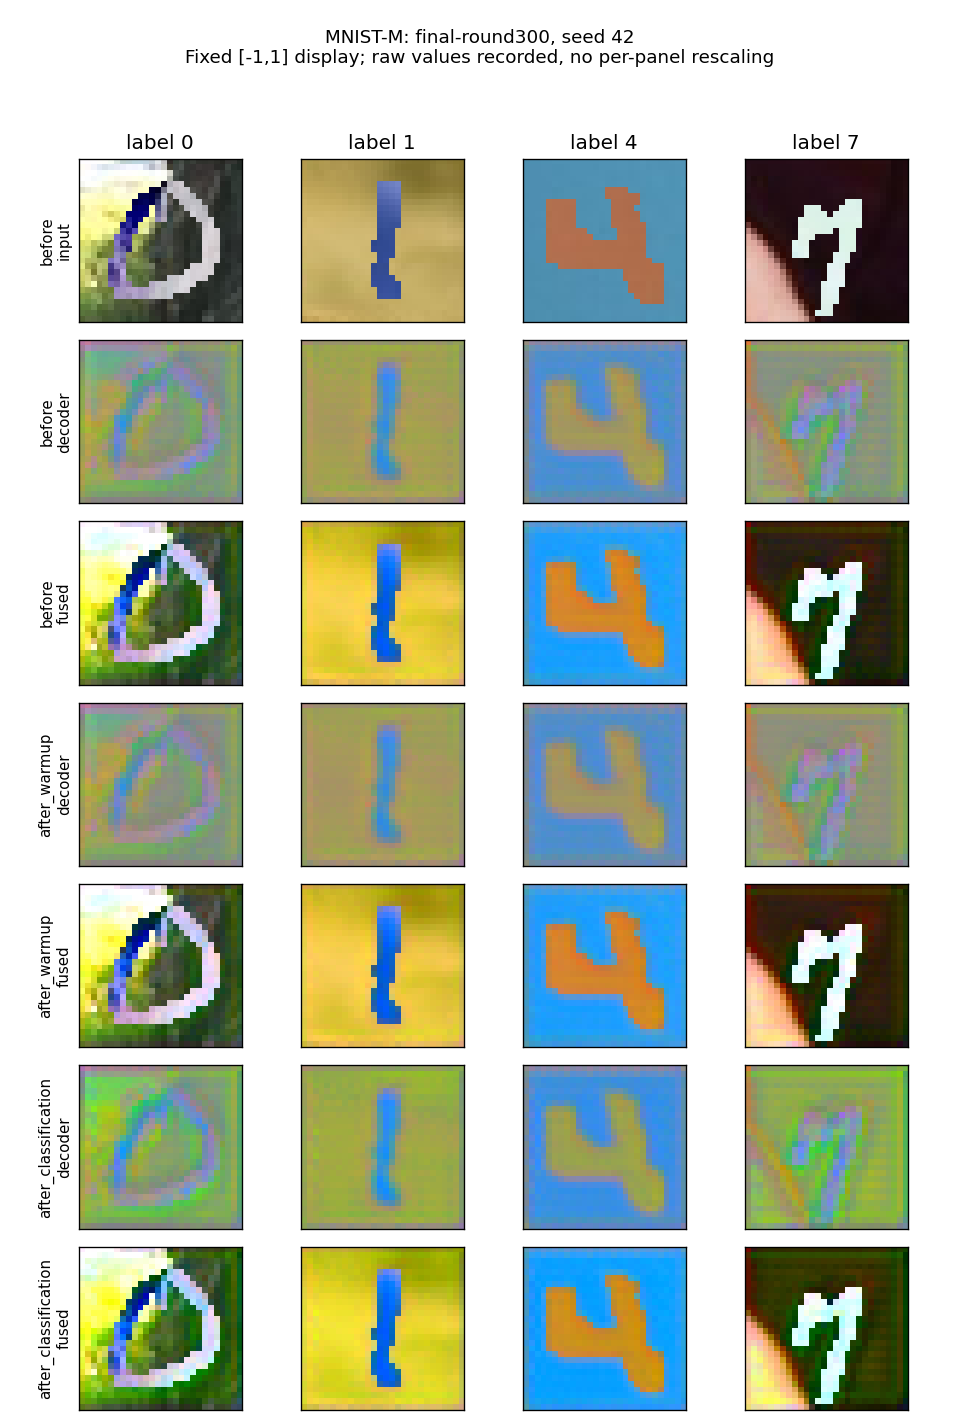
\includegraphics[width=.56in,trim=47.4bp 227.4bp 430.2bp 531.0bp,clip]{figures/digits/final-round300-MNIST-M.png} \\[-2pt]
\raisebox{.20in}{\scriptsize\shortstack[r]{After classification\\decoder}} & 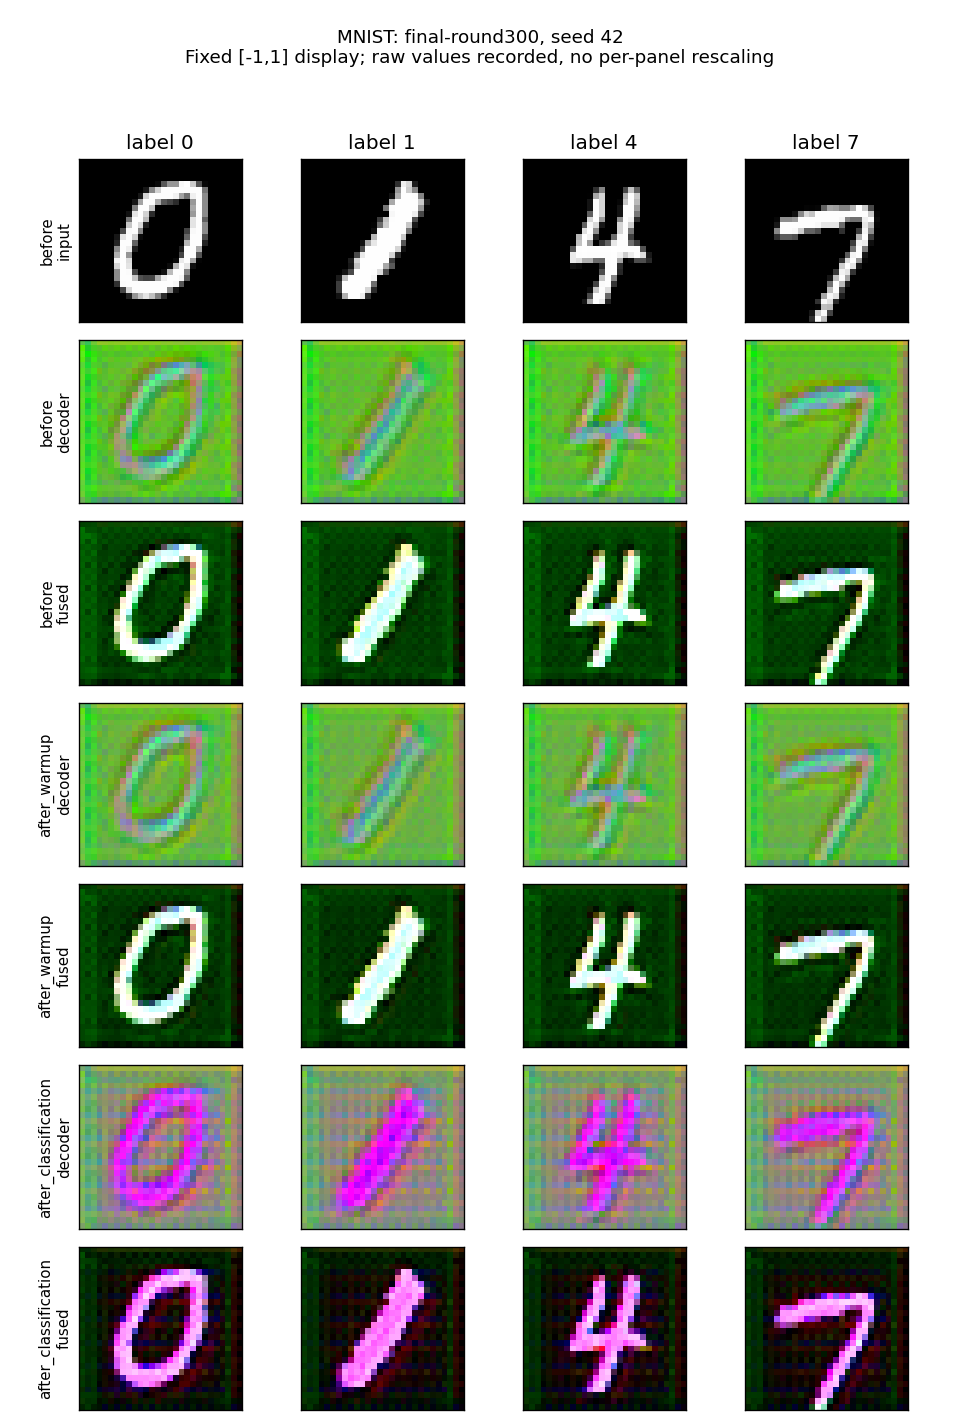
\includegraphics[width=.56in,trim=47.4bp 118.8bp 430.2bp 639.6bp,clip]{figures/digits/final-round300-MNIST.png} & 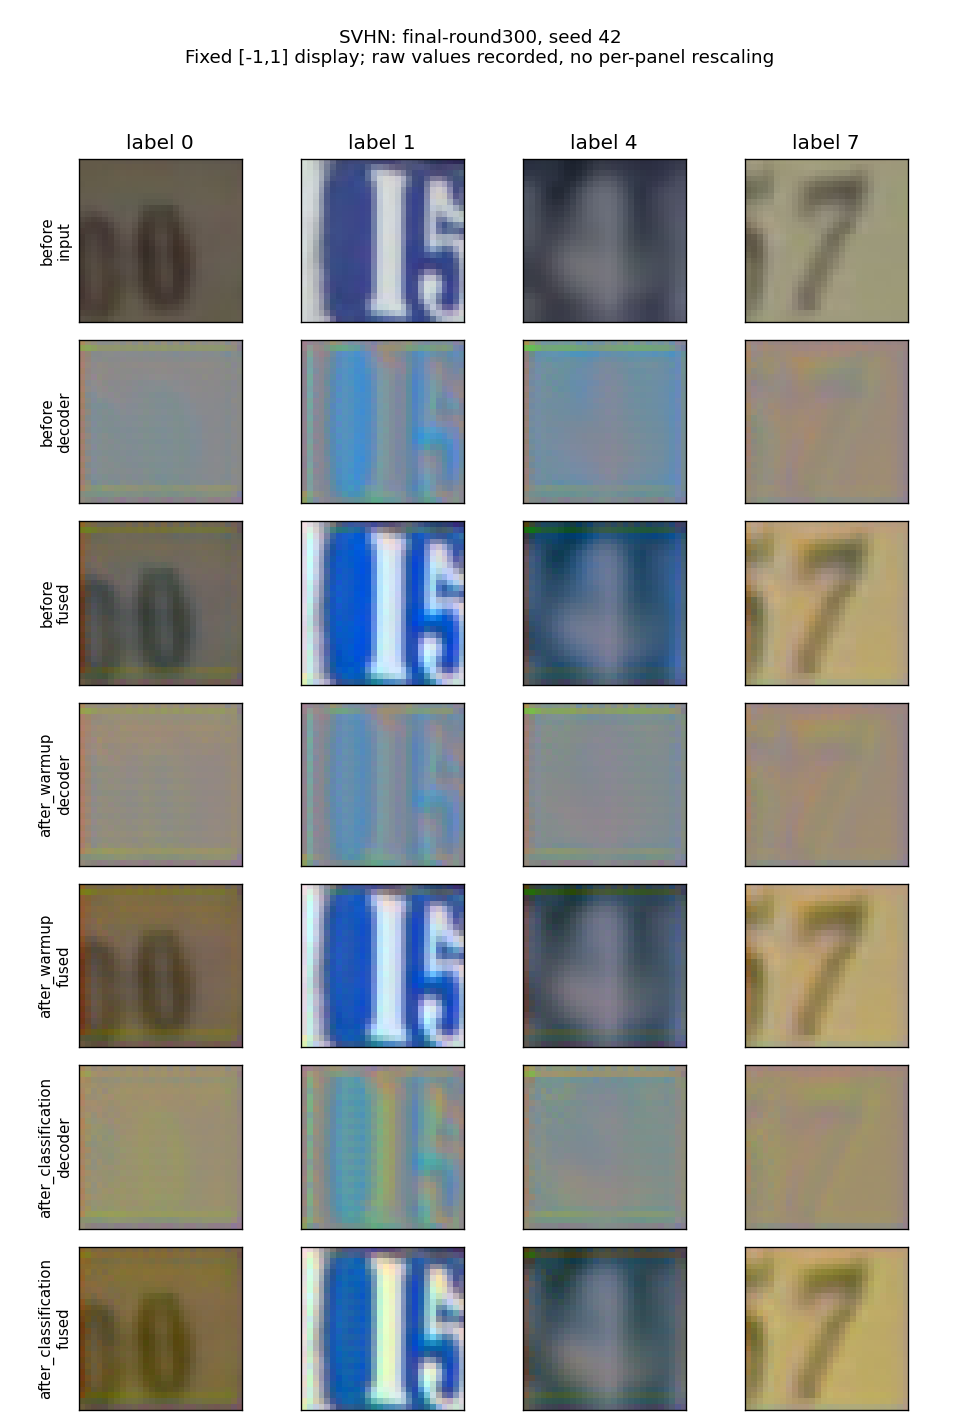
\includegraphics[width=.56in,trim=47.4bp 118.8bp 430.2bp 639.6bp,clip]{figures/digits/final-round300-SVHN.png} & 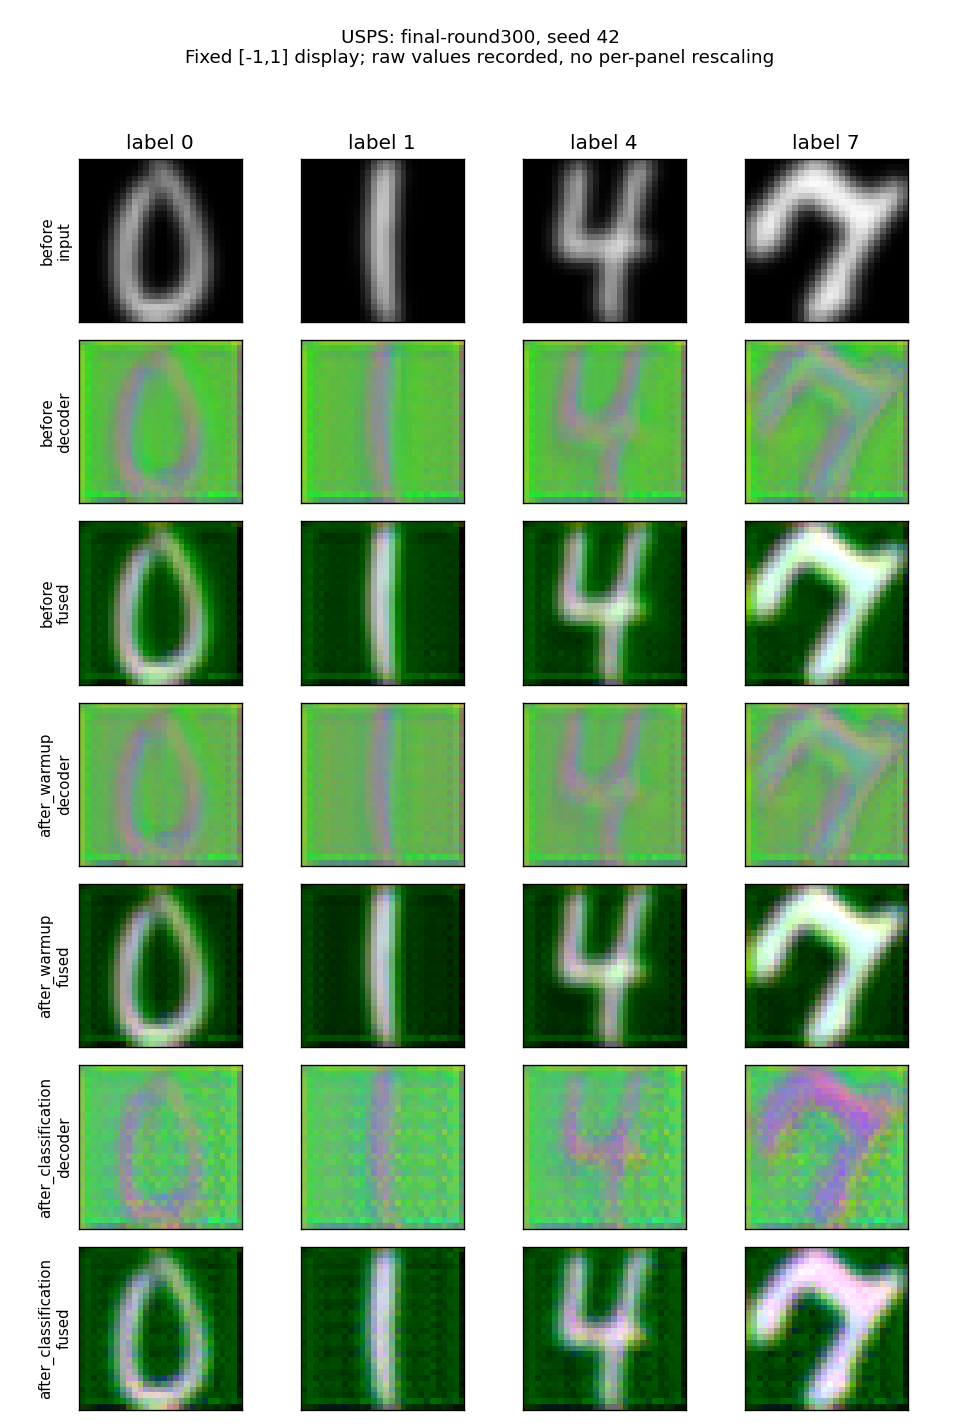
\includegraphics[width=.56in,trim=47.4bp 118.8bp 430.2bp 639.6bp,clip]{figures/digits/final-round300-USPS.png} & 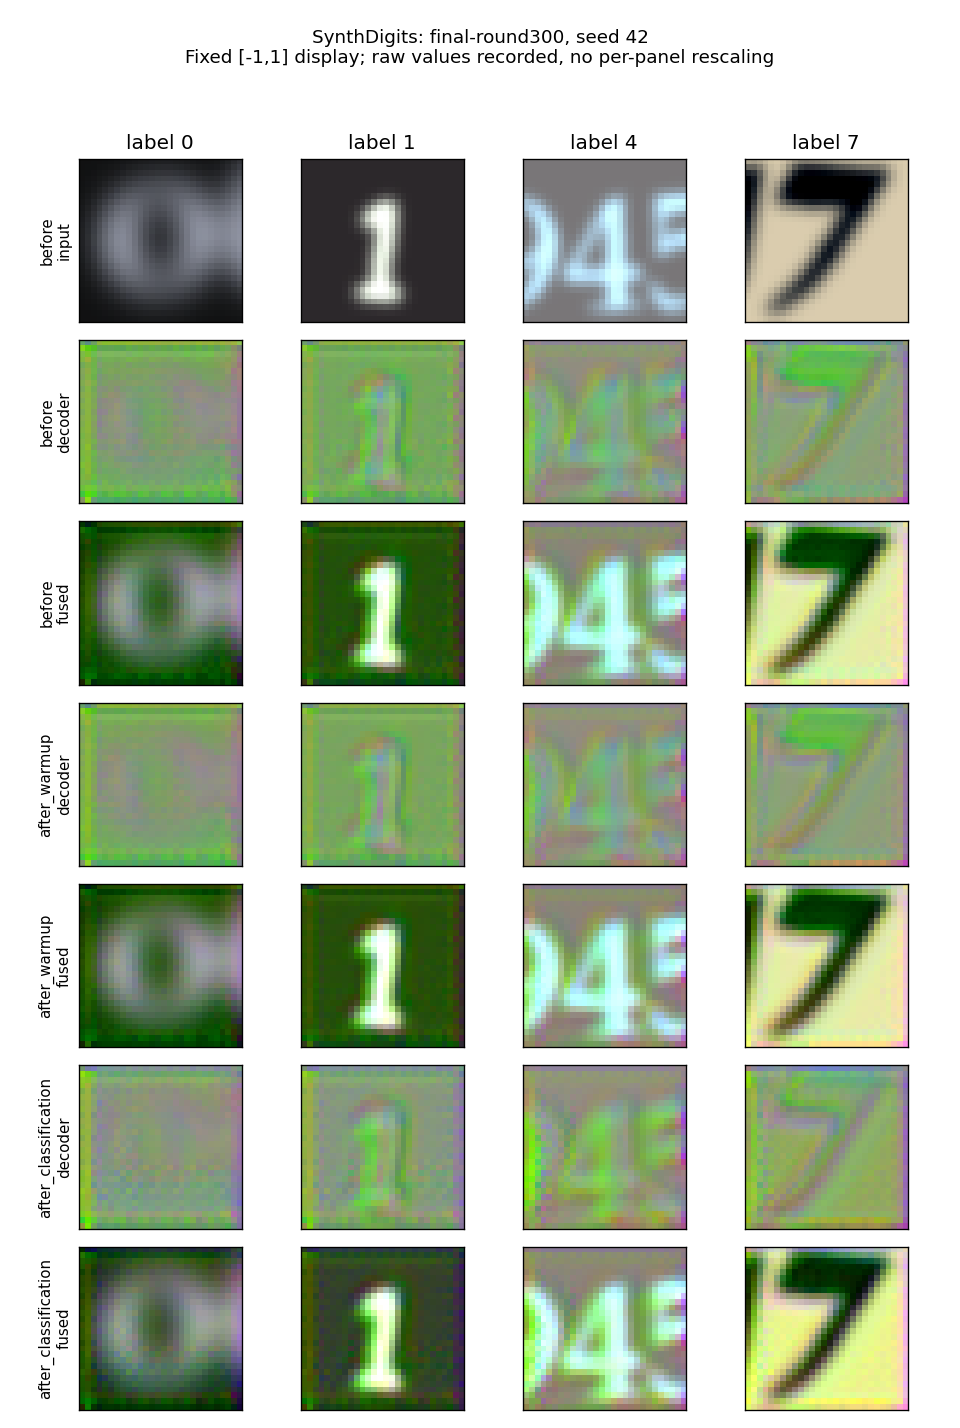
\includegraphics[width=.56in,trim=47.4bp 118.8bp 430.2bp 639.6bp,clip]{figures/digits/final-round300-SynthDigits.png} & 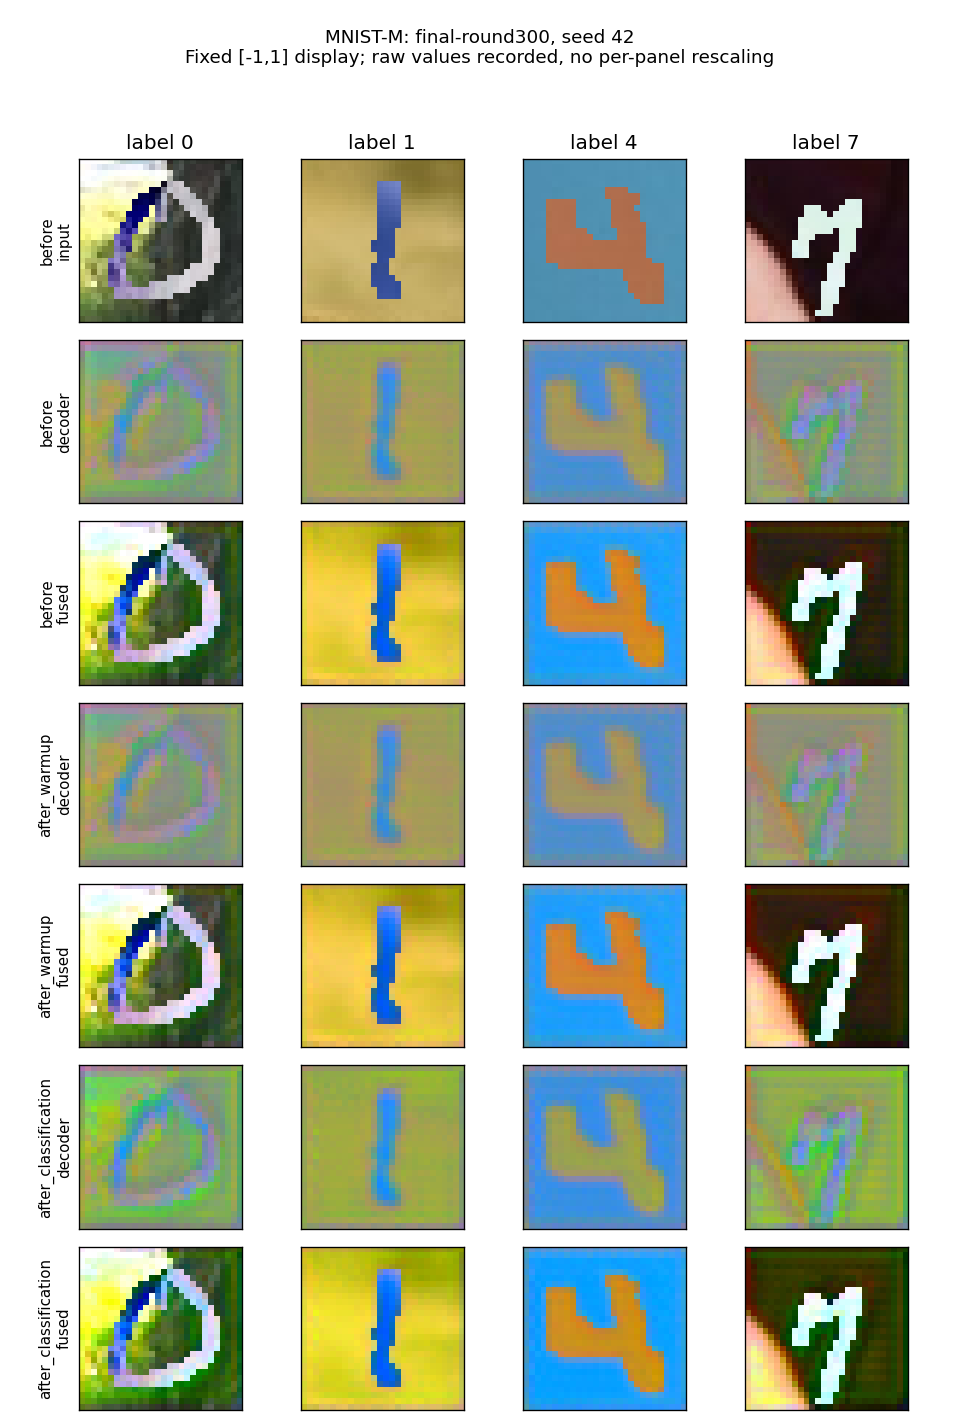
\includegraphics[width=.56in,trim=47.4bp 118.8bp 430.2bp 639.6bp,clip]{figures/digits/final-round300-MNIST-M.png} \\[-2pt]
\raisebox{.20in}{\scriptsize\shortstack[r]{After classification\\fused}} & 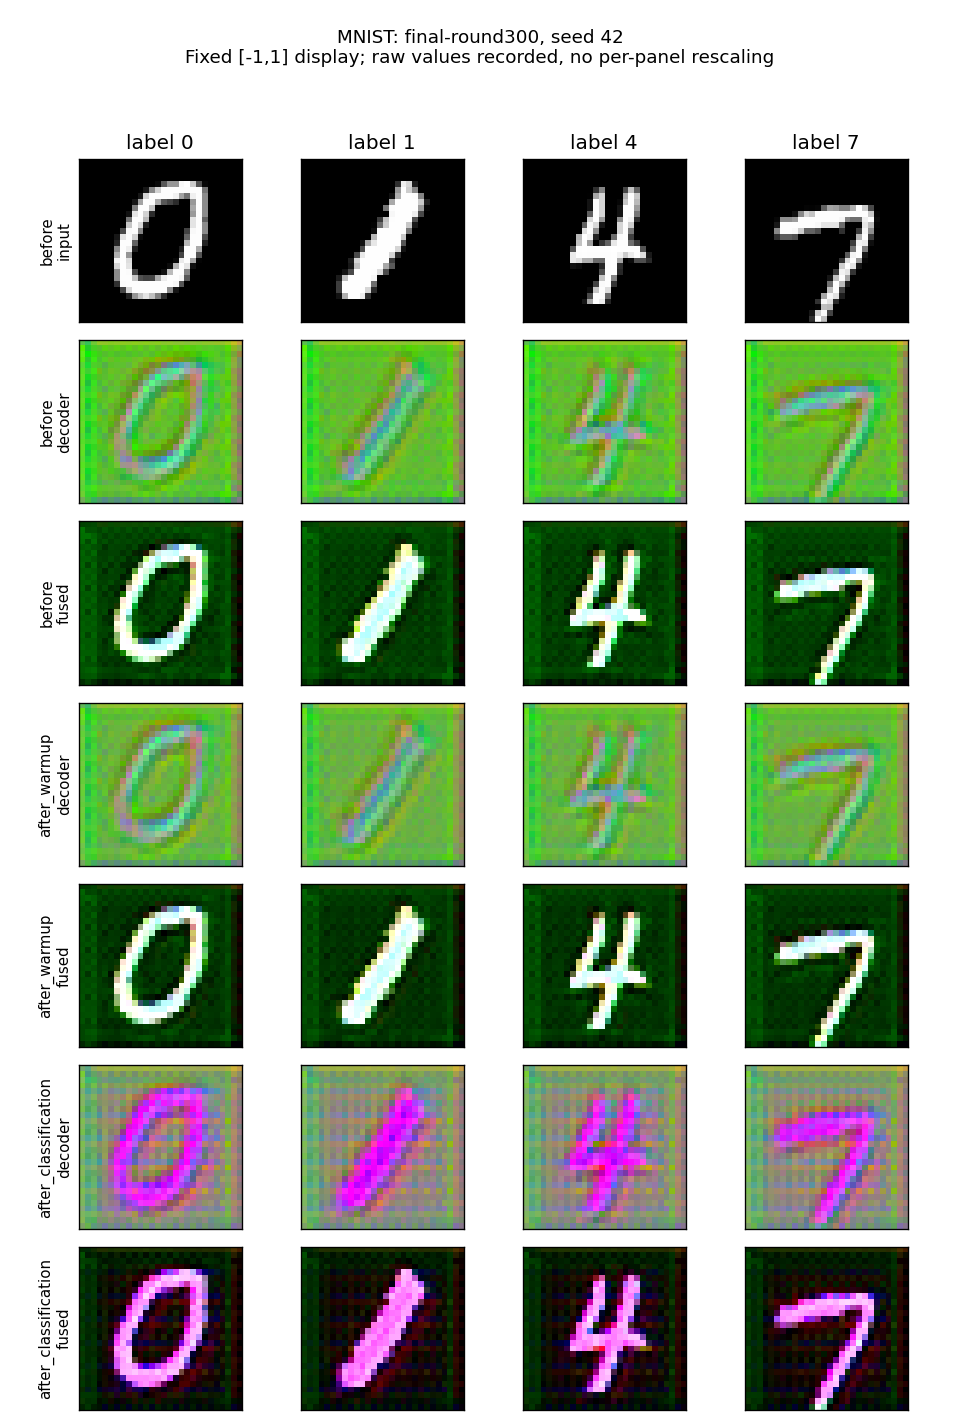
\includegraphics[width=.56in,trim=47.4bp 9.6bp 430.2bp 748.8bp,clip]{figures/digits/final-round300-MNIST.png} & 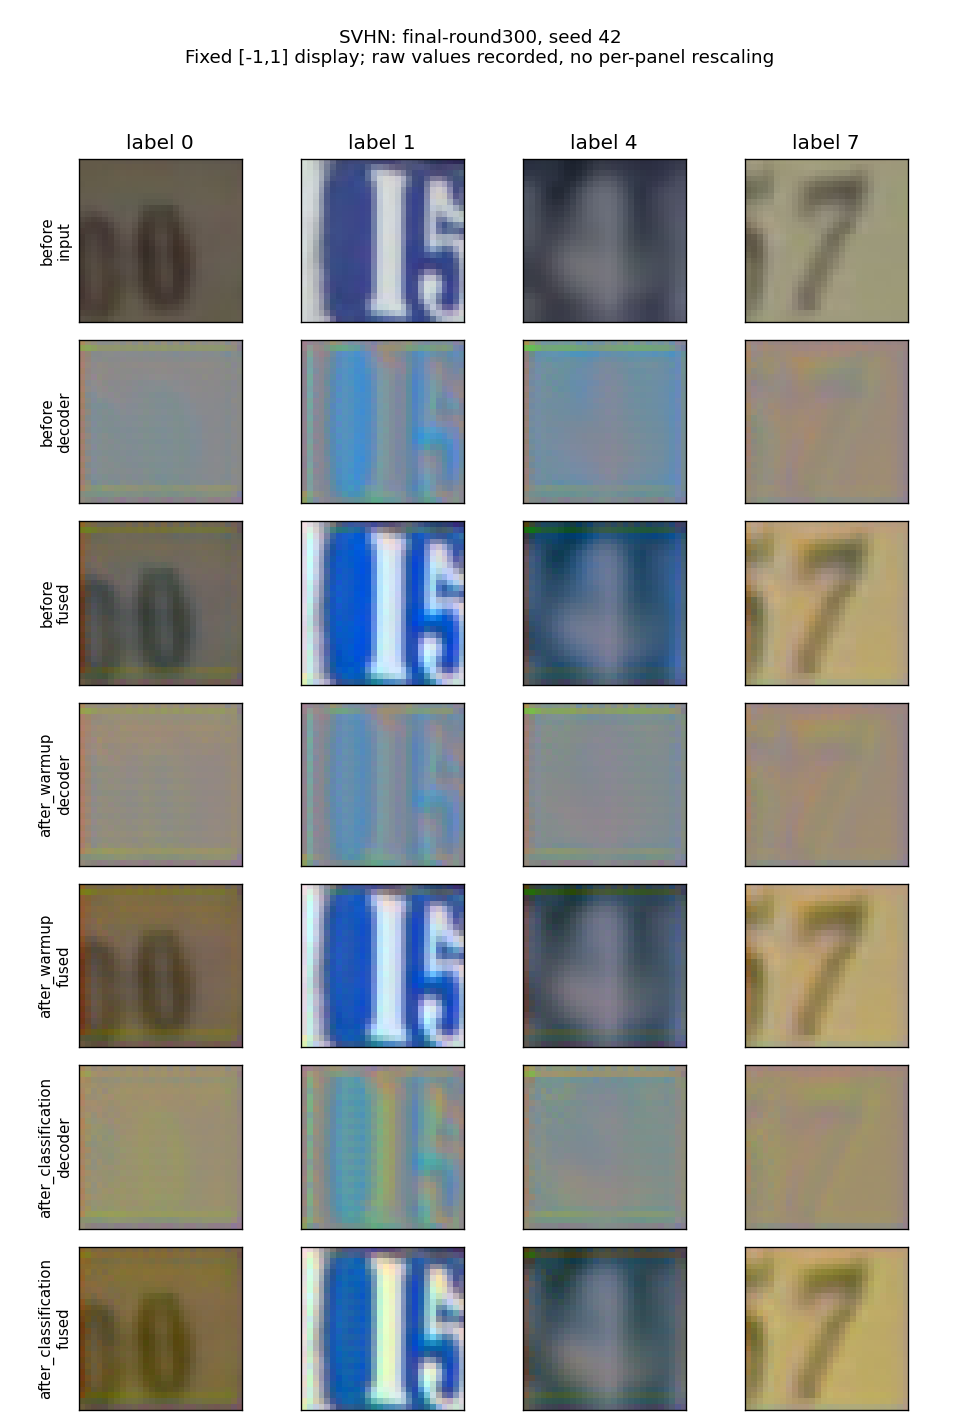
\includegraphics[width=.56in,trim=47.4bp 9.6bp 430.2bp 748.8bp,clip]{figures/digits/final-round300-SVHN.png} & 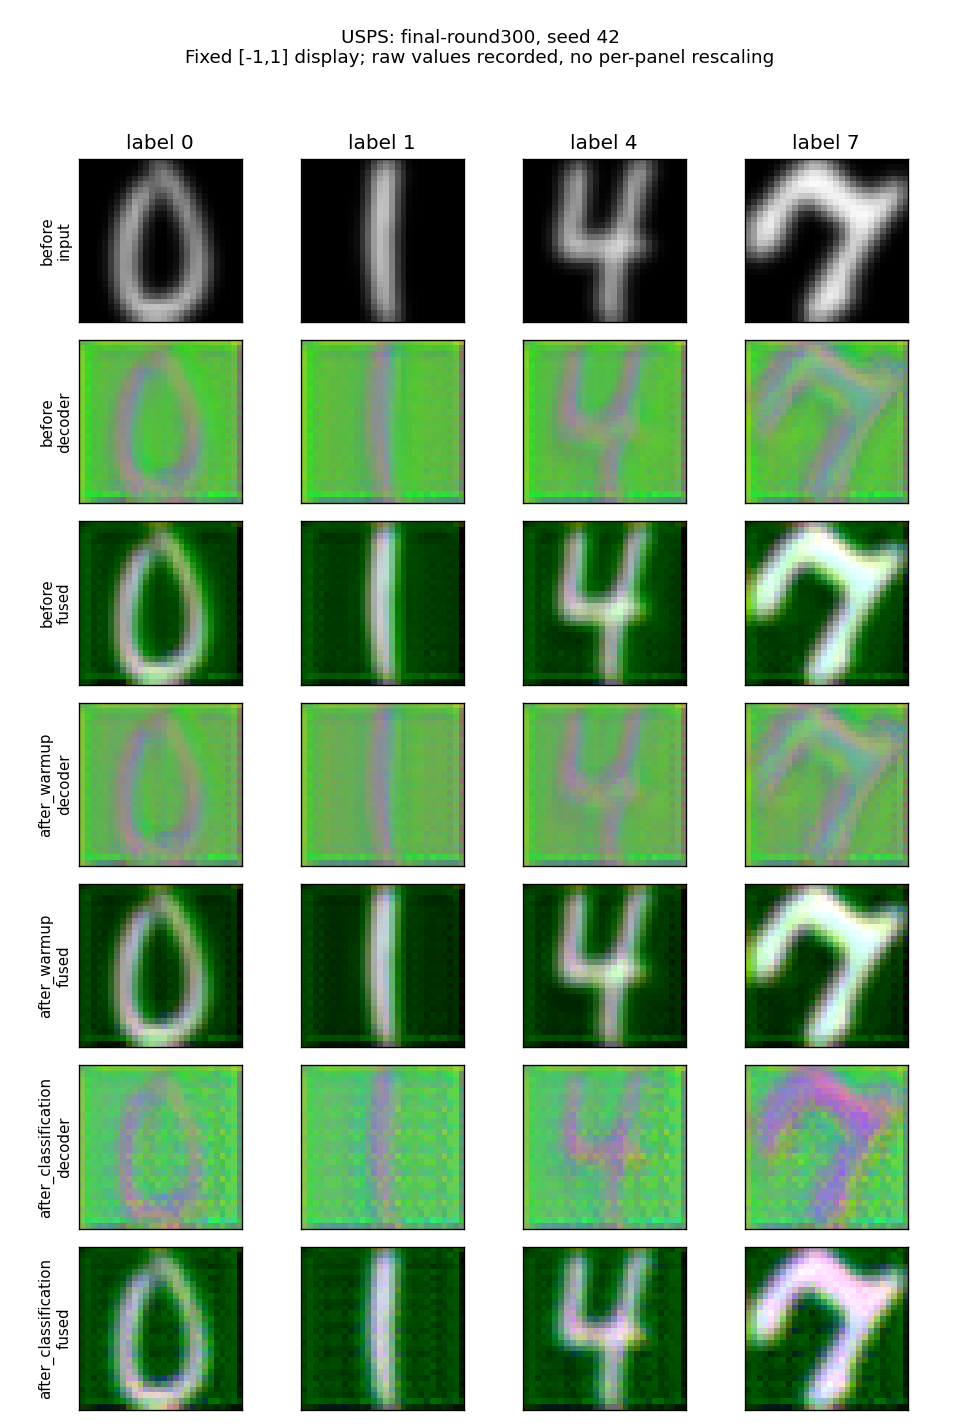
\includegraphics[width=.56in,trim=47.4bp 9.6bp 430.2bp 748.8bp,clip]{figures/digits/final-round300-USPS.png} & 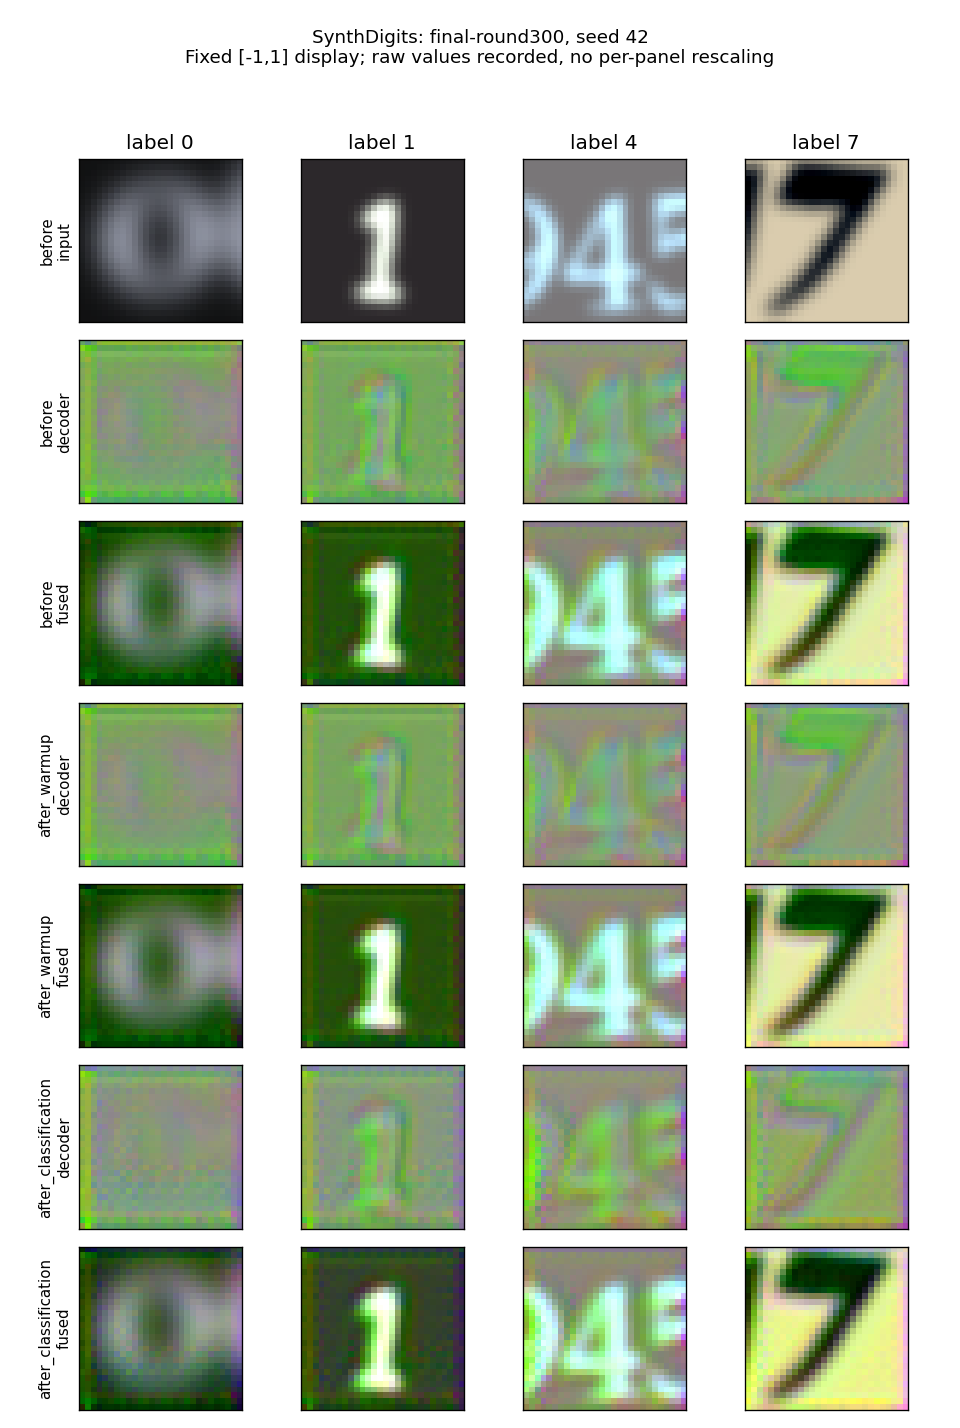
\includegraphics[width=.56in,trim=47.4bp 9.6bp 430.2bp 748.8bp,clip]{figures/digits/final-round300-SynthDigits.png} & 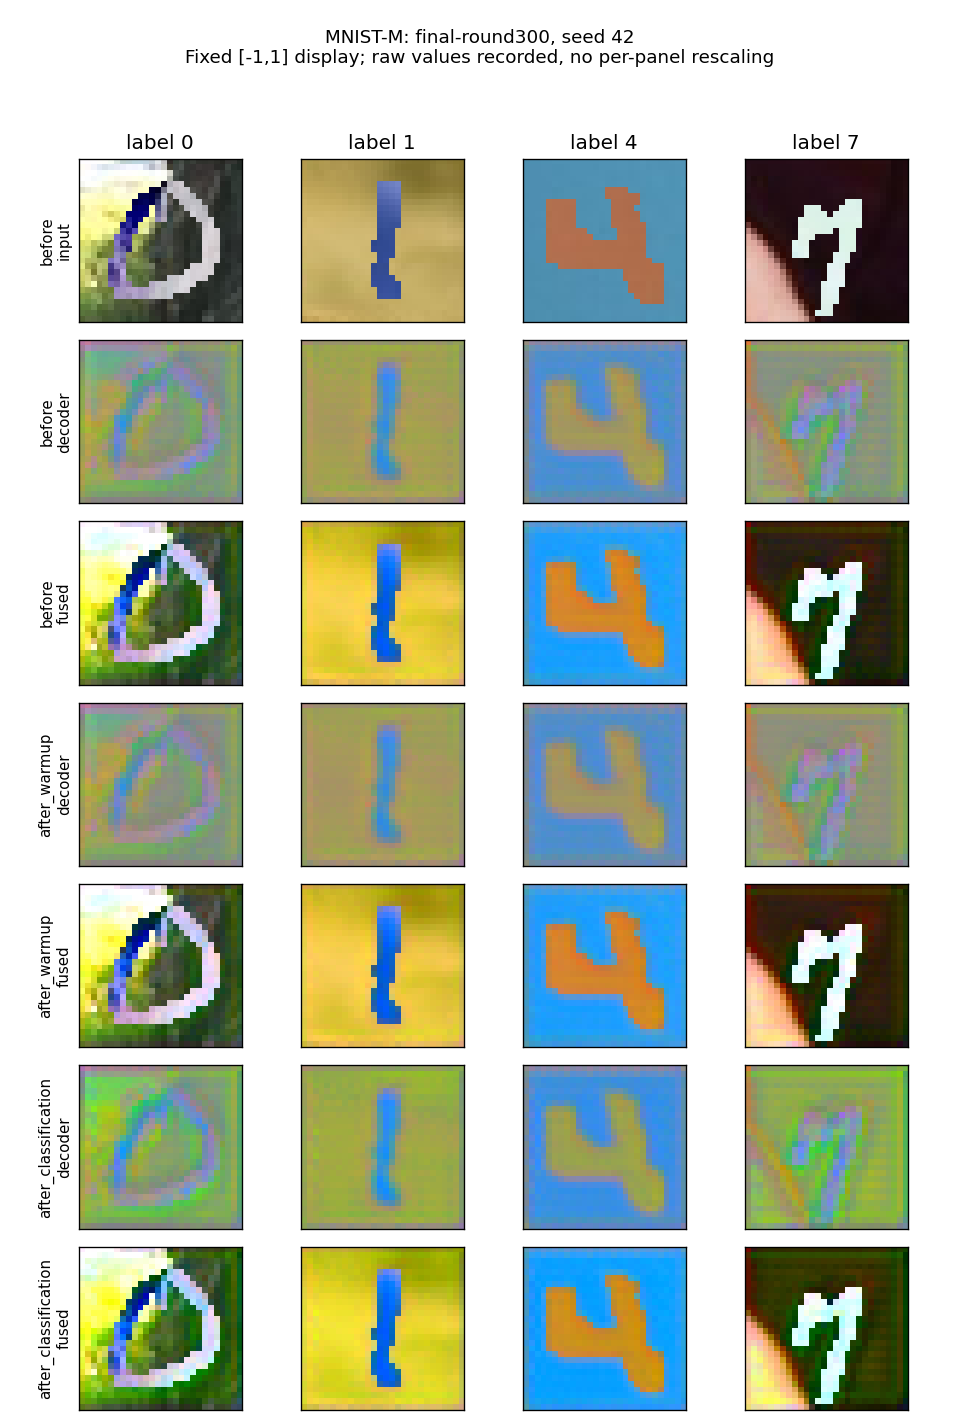
\includegraphics[width=.56in,trim=47.4bp 9.6bp 430.2bp 748.8bp,clip]{figures/digits/final-round300-MNIST-M.png} \\[-2pt]
\end{tabular}
\caption{Digits decoder probes from the final checkpoint, seed 42. Each column uses the first preselected class-0 example in that domain; the same example is shown throughout its local replay. Rows show the input and the decoder and fused outputs before adaptation, after warm-up, and after classification. All panels retain the fixed display range $[-1,1]$ of the archived grids; clipping is applied only for visualization, without panel-specific rescaling. Quantitative measurements use the raw, unclipped outputs.}
\label{fig:digits_decoder_probe}
\end{figure*}
